\documentclass[a4paper, 11pt, table]{article}

\usepackage[utf8]{inputenc}
\usepackage[english]{babel}
\usepackage[table]{xcolor}
\usepackage{graphicx}
\usepackage{tikz}
\usetikzlibrary{calc}
\usepackage{float}
\usepackage{pifont,mdframed}
\usepackage{subfig}
\usepackage{amsmath}
\usepackage{pdfpages}
\usepackage{siunitx}
\sisetup{
    group-digits=true,
    group-separator={\,},
}
\usepackage{caption}
\usepackage{pifont}
\usepackage{footnote}
\makesavenoteenv{tabular}
\usepackage{pgfplots}
\usetikzlibrary{pgfplots.groupplots}
\usetikzlibrary{matrix}
\usepackage{booktabs}
\usepackage{csquotes}
\usepackage{afterpage}
\usepackage{pdflscape}
\usetikzlibrary{patterns}

\usepackage{hyperref}


\usepackage[backend=biber,sorting=none]{biblatex}
\addbibresource{references.bib}

% http://tex.stackexchange.com/questions/12703/how-to-create-fixed-width-table-columns-with-text-raggedright-centered-raggedlef
\usepackage{array}
\newcolumntype{L}[1]{>{\raggedright\let\newline\\\arraybackslash\hspace{0pt}}m{#1}}
\newcolumntype{C}[1]{>{\centering\let\newline\\\arraybackslash\hspace{0pt}}m{#1}}
\newcolumntype{R}[1]{>{\raggedleft\let\newline\\\arraybackslash\hspace{0pt}}m{#1}}


\definecolor{Gray}{gray}{0.9}
\definecolor{LabelColor}{gray}{0.0}
\definecolor{clno}{RGB}{212, 59, 59}
\definecolor{clyes}{RGB}{12, 150, 12}
\definecolor{linux}{RGB}{255, 186, 249}
\definecolor{windows}{RGB}{186,215, 255}
\definecolor{macos}{gray}{0.9}  
\definecolor{clstackoverflow}{HTML}{FE7A15}  
\definecolor{clgithub}{HTML}{4078C0} 

\definecolor{lblue}{HTML}{4286F4} 
\definecolor{lgreen}{HTML}{30A349} 
\definecolor{lred}{HTML}{F44242} 
\definecolor{lpurple}{HTML}{DC42F4} 
\definecolor{lyellow}{HTML}{F4D742}


\newcommand{\cmark}{\ding{51}}%
\newcommand{\xmark}{\ding{55}}%
\newcommand{\ymark}{\textcolor{clyes}{\cmark}}%
\newcommand{\nmark}{\textcolor{clno}{\xmark}}%

% Roman numerals
\newcommand{\rom}[1]{\uppercase\expandafter{\romannumeral #1\relax}}

% plots
% https://www.sharelatex.com/learn/Pgfplots_package
\pgfplotsset{width=10cm,compat=1.9}
%\usepgfplotslibrary{external} 
%\tikzexternalize

% short for multicolumn-centered
\newcommand{\mcc}[1]{\multicolumn{1}{c}{#1}}

% http://tex.stackexchange.com/questions/2441/how-to-add-a-forced-line-break-inside-a-table-cell
\newcommand{\specialcell}[2][c]{%
  \begin{tabular}[#1]{@{}c@{}}#2\end{tabular}}

\graphicspath{ {img/} }

% warning environment
% It should not be included in final report
% http://tex.stackexchange.com/questions/8689/how-to-create-a-warning-box-like-this-see-the-figure-to-get-the-idea
\newenvironment{warning}
  {\par\begin{mdframed}[linewidth=2pt,linecolor=red]%
    \begin{list}{}{\leftmargin=1cm
                   \labelwidth=\leftmargin}\item[\Large\ding{43}]}
  {\end{list}\end{mdframed}\par}

\title{Convolutional neural networks for classification of transmission electron microscopy imagery}

\author{Sergii Gryshkevych}
\date{\today}

\begin{document}

% remove page numbering
% http://tex.stackexchange.com/questions/54333/no-page-numbering
\pagenumbering{gobble}

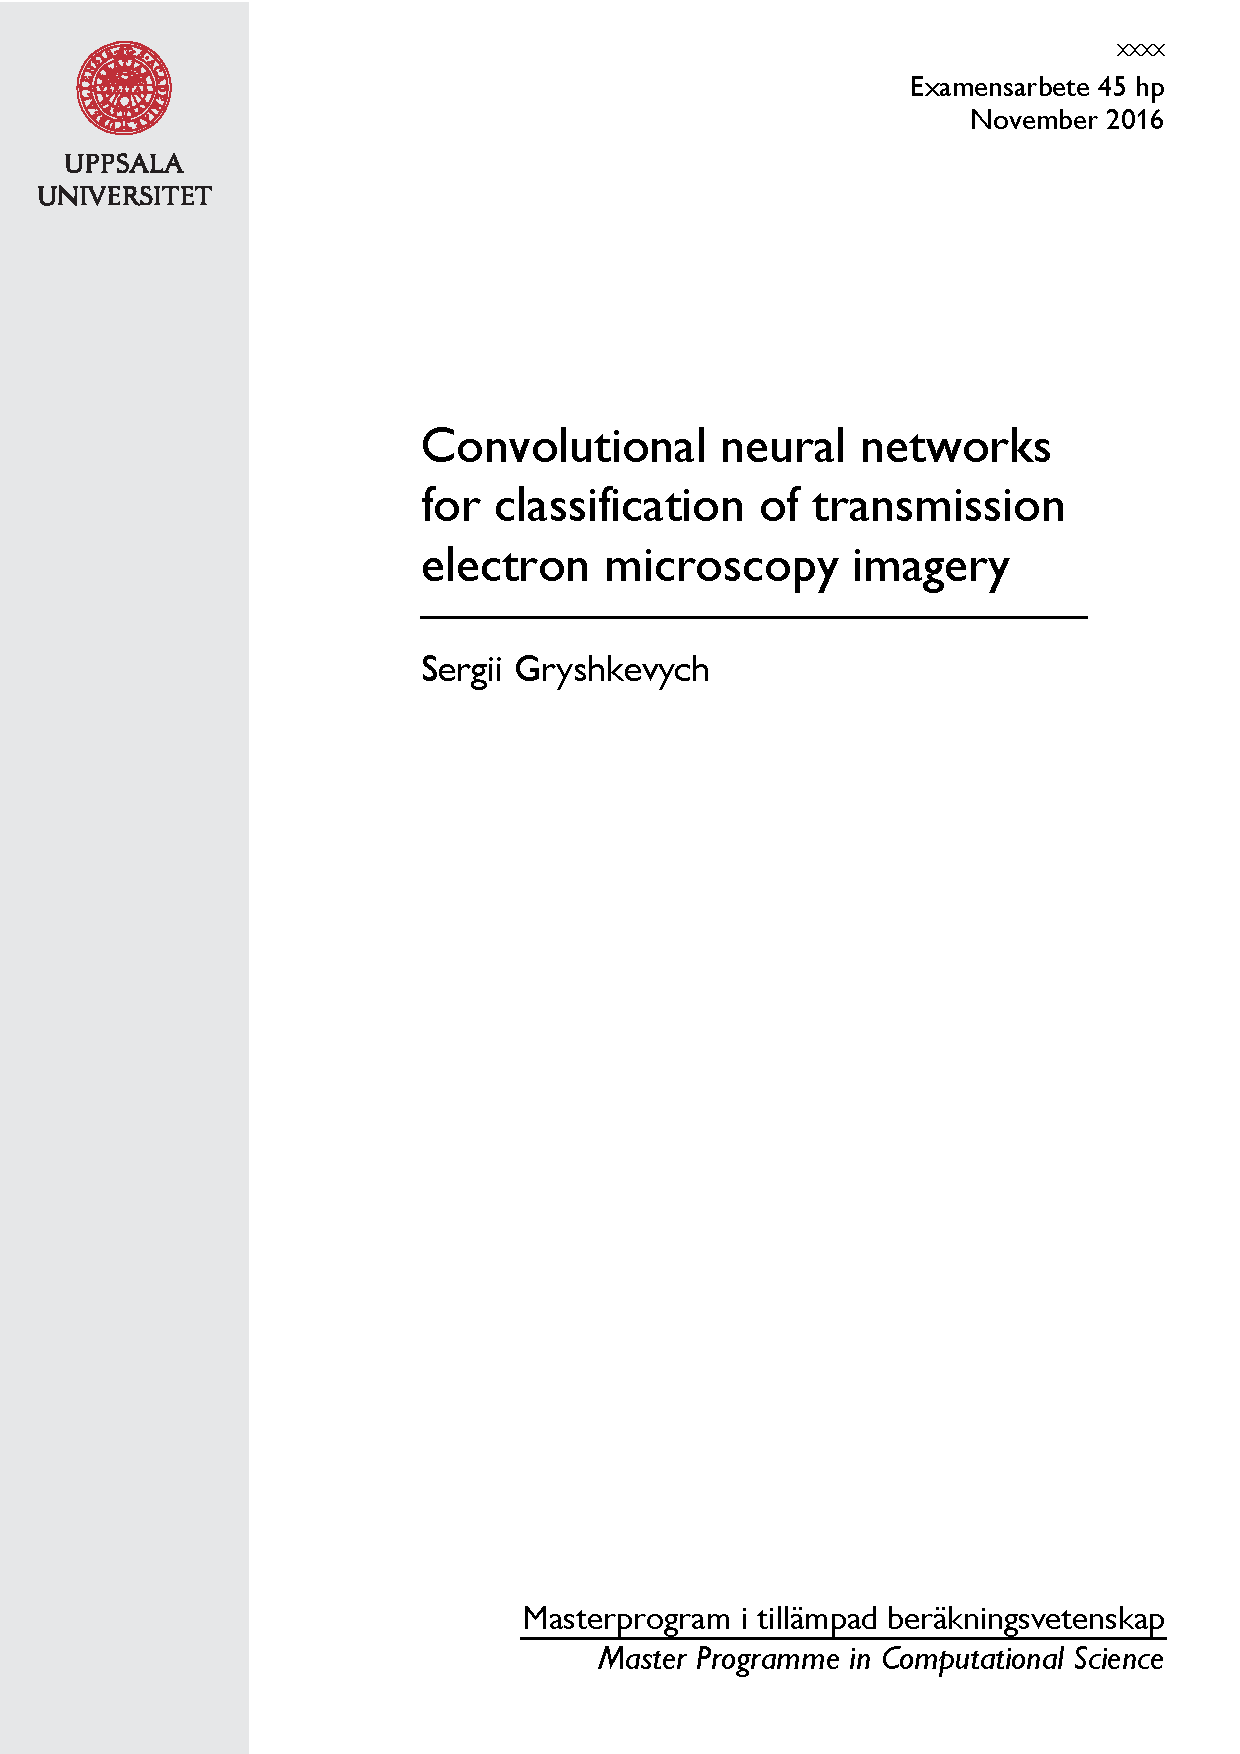
\includepdf{./resources/first_page.pdf}
\newpage\phantom{}
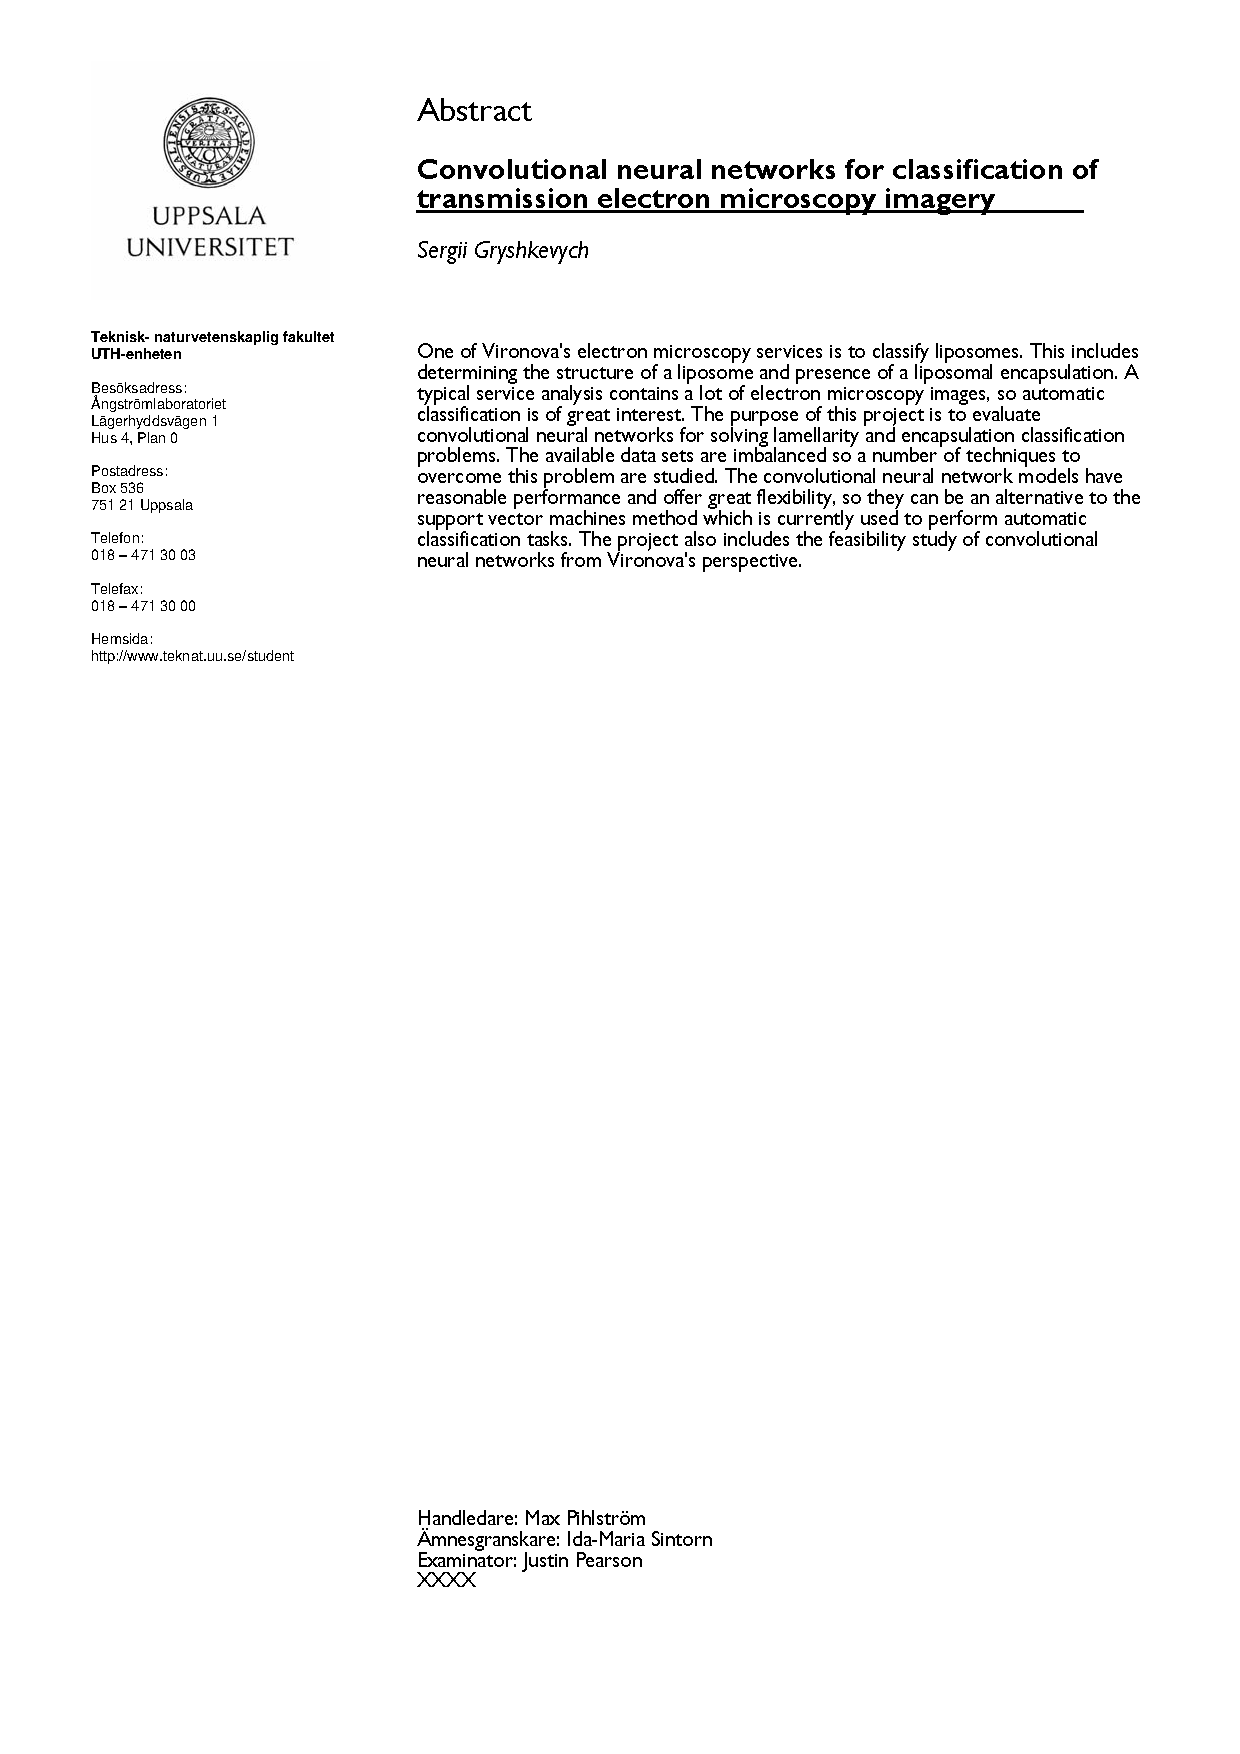
\includepdf{./resources/abstract.pdf}
\newpage\phantom{}
\newpage\phantom{}

% Abstract page 
% http://pdf.teknik.uu.se/pdf/abstract.php
% One of Vironova's electron microscopy services is to classify liposomes. This includes determining the structure of a liposome and presence of a liposomal encapsulation. Vironova has a lot of electron microscopy images so automatic classification is of great interest. The purpose of this project is to evaluate convolutional neural networks for solving lamellarity and encapsulation classification problems. The available data sets are imbalanced so a number of techniques to overcome this problem are studied. The convolutional neural network models have reasonable performance and offer great flexibility, so they can be an alternative to the support vector machines method which is currently used to perform automatic classification tasks.

% Arabic page numbers (and reset to 1)
\pagenumbering{arabic}
\tableofcontents

\section{Introduction}
Vironova is a Swedish Biotech company that supplies hardware and software solutions for advanced electron microscopy (EM), image analysis, nano-characterization and viral clearance testing~\cite{virnonva_linkedin}. Vironova's analyses contain a lot of EM images and many its tasks involve a classification step, therefore automatic classification is of great interest. Currently automatic classification is performed by means of support vector machines (SVM)~\cite{Boser:1992:TAO:130385.130401}, which demonstrates reasonable performance. On the other hand SVM operates on features extracted from the images rather than on raw pixel data. Determining a set of features that describes differences between classes is a non-trivial task that requires expert knowledge. This motivates interest in methods that operate on raw pixel data and are capable of learning image features themselves during training. 

Convolutional neural networks (CNNs)~\cite{LeCun1986} is one of such methods. CNN are designed to recognize visual patterns directly from pixel data with minimal preprocessing. One of the first successful applications of CNN to a large data set was recognition of handwritten digits~\cite{41400} in the end of 80s'. Since then CNN has demonstrated excellent results in wide range of problems~\cite{NIPS2012_4824, DBLP:journals/corr/LinCY13}. For example CNN are used for segmentation~\cite{DBLP:journals/corr/ShelhamerLD16, Ronneberger2015} and for classification~\cite{NIPS2012_4824, DBLP:journals/corr/abs-1202-2745} tasks.

The goal of this project is to study and evaluate the suitability of using CNNs for automatic classification of electron microscopy (EM) images. CNN models are evaluated by benchmarking against SVM for selected problems. This project also encompasses prospecting the role of CNN technology for the Vironova EM services both as a method for automatic classification included in the software as well as being a research tool (e.g., for identifying useful particle features). This includes discussion on library licenses, operating system availability, performance and community support.

\section{Problem description}
\label{sec:problem_description}
One of Vironova's electron microscopy services is to classify different types of liposomes\footnote{A liposome is a spherical vesicle having at least one lipid bilayer~\cite{betageri1993liposome}. Liposomes were first described in 1964 by A.D. Bangham and R.W. Thorne and G. Weissman. They suggested the name "liposome"~\cite{betageri1993liposome}. Liposomes can be classified into different types according to numerous features such as but not limited to size, number of lamellae, composition, shape, production method, etc. The classification of liposomes was first presented at a meeting of New York Academy of Science~\cite{liposomes1978}.}. This includes determining:
\begin{itemize}
\item The structure of the liposome.
\item The presence of liposomal encapsulation of, for example or doxorubicin.
\end{itemize}

Let us call these two problems as \textit{Lamellarity} and \textit{Encapsulation}.\medskip

\textbf{Lamellarity}. The term lamellarity refers to the number of lamellae. Lamella, in cell biology, is used to describe numerous plate or disc-like structures at both a tissue and cellular level~\cite{cammack2006oxford}. According to the number of lamellae liposomes can be \textit{unilamellar} (single lamella) and \textit{multilamellar} (multiple lamellae). In addition, an \textit{uncertain} class is introduced because in some cases it is almost impossible to be certain about  the lamellarity class. Liposomes can for example overlap each other. Another issue to keep in mind is that samples are usually delivered frozen, so liposomes may be partly covered with pieces of ice that result in large black blobs in the EM images. Figure~\ref{fig:lamellarity_problem} illustrates examples of liposomes from each class.

\begin{figure}[H]
\centering
\begin{tabular}{ccc}
	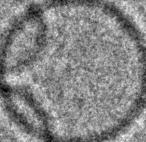
\includegraphics[height=2cm, keepaspectratio]{problem_description/lamellarity/uni} & 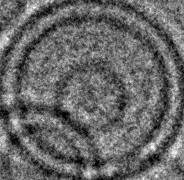
\includegraphics[height=2cm, keepaspectratio]{problem_description/lamellarity/multi} & 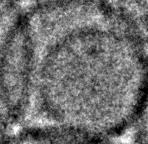
\includegraphics[height=2cm, keepaspectratio]{problem_description/lamellarity/uncertain} \\
	Unilamellar & Multilamellar & Uncertain \\[6pt]
\end{tabular}
\caption{Lamellarity problem, 3 classes}
\label{fig:lamellarity_problem}
\end{figure}

Table~\ref{table:lamellarity_data_set} presents the lamellarity problem data set which contains $\num{14169}$ liposome objects. All images in this data set have been manually classified by an expert into three classes.

\begin{center}
\captionof{table}{Lamellarity problem}
\label{table:lamellarity_data_set}
\begin{tabular}{lrr}
\toprule
Unilamellar & \num{12368} & 87.29\% \\ 
Multilamellar & \num{1717} & 12,12\% \\ 
Uncertain & \num{84} & 0,59\% \\ 
\end{tabular} 
\end{center}


\textbf{Encapsulation}. Liposomes can be used as vehicles for drug delivery to various destinations in the human body~\cite{betageri1993liposome}. A crucial part of testing this approach is to measure how many liposomes responded to drugs encapsulation and can carry them further. In the encapsulation problem liposomes are classified between the following classes: \textit{full}, i.e. liposomes that received the drug substance; \textit{empty}, i.e. liposomes that remained empty after the encapsulation attempt. As in the lamellarity problem, the \textit{uncertain} class is introduced with the same motivation. Figure~\ref{fig:encapsulation_problem} illustrates different classes of the encapsulation problem. Table~\ref{table:encapsulation_dataset} presents the encapsulation problem data set which contains $\num{24918}$ EM objects. Images in this data set are also manually classified into three classes.

\begin{figure}[H]
\centering
\begin{tabular}{ccc}
	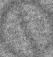
\includegraphics[height=2cm, keepaspectratio]{problem_description/packiging/full} & 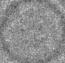
\includegraphics[height=2cm, keepaspectratio]{problem_description/packiging/empty} & 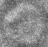
\includegraphics[height=2cm, keepaspectratio]{problem_description/packiging/uncertain} \\
	Full & Empty & Uncertain \\[6pt]
\end{tabular}
\caption{Encapsulation problem, 3 classes}
\label{fig:encapsulation_problem}
\end{figure}


\begin{center}
\captionof{table}{Encapsulation problem}
\label{table:encapsulation_dataset}
\begin{tabular}{lrr}
\toprule
Full & \num{24255} & 97.34\% \\ 
Uncertain & \num{502} & 2.01\% \\ 
Empty & \num{161} & 0.65\% \\ 
\end{tabular} 
\end{center}

\section{The data}
\label{sec:dataset}
The data for this project is provided by Vironova AB. The data consists of two data sets corresponding to the lamellarity and the encapsulation problems respectively. Both data sets contain grayscale EM image cut outs of particles and a number of computed image features.

Each image depicts exactly one liposome object which is located in the center of the image. In addition each image contains liposome's surrounding that goes 50 pixels in each direction. The effect of the liposome surrounding on the classifier performance is described later in this report. Corresponding particle masks are also provided. All liposomes have different sizes and so do corresponding images. The size of the liposome might be an important feature that potentially could help to describe the differences between the classes.  Figure~\ref{fig:img_size_scatter_plot} shows scatter plots where the axes correspond to image width and height in pixels. Figure~\ref{fig:img_size_per_class} demonstrates image size distribution inside each class.

\begin{figure}[H]
\centering
\begin{tabular}{cc}
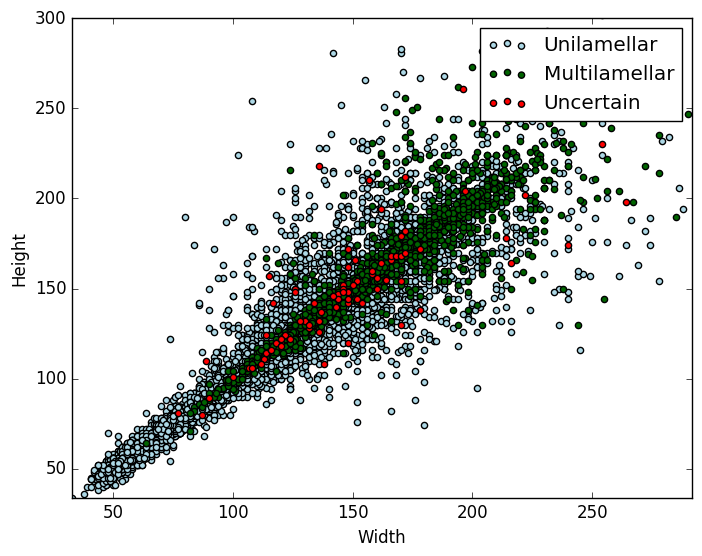
\includegraphics[scale=0.32]{img_size/lamellarity/scatter_plot_width_height.png} & 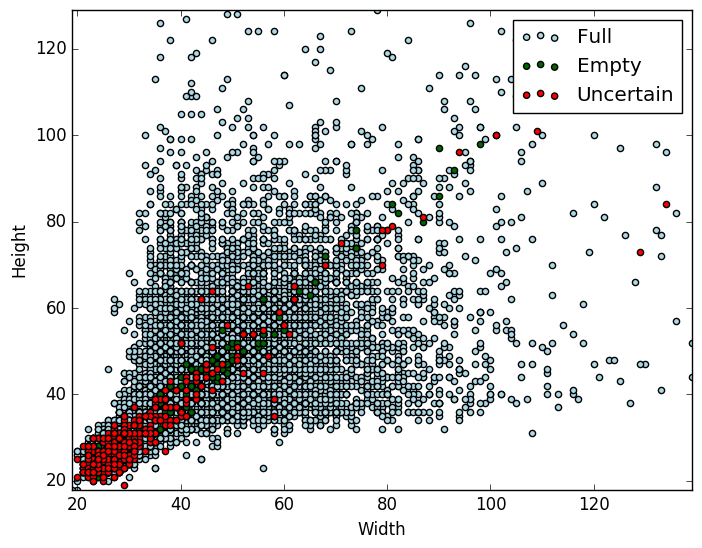
\includegraphics[scale=0.32]{img_size/encapsulation/scatter_plot_width_height.png}
\end{tabular}
\caption{Scatter plots of image sizes (best viewed in color): lamellarity data set is shown to the leftand encapsulation to the right. Width and height units are in pixels.}
\label{fig:img_size_scatter_plot}
\end{figure}

%\pagebreak
\begin{minipage}{\linewidth}
Both data sets contain the following features:
\begin{itemize}
\item \textbf{Maximum width} in nanometres. If the particle is an ellipse, then it is a diameter along the largest axis. If the particle is a polygon, then it is the maximum value of distance transform of particle mask.

\item \textbf{Diameter} in pixels. If the particle is an ellipse, then it is a diameter along the largest axis. If the particle is a polygon, then it is the greatest distance between any two vertices. 

\item \textbf{Length} is defined as diameter converted to nanometre units.

\item \textbf{Histogram}: histogram of pixel intensity values, 32 bins.

\item \textbf{Moments}: image moments $\mu_{20}$, $\mu_{02}$, $\mu_{30}$, $\mu_{03}$ as defined in~\cite{1057692}. 

\item \textbf{Radial Density Profile} is a 2D array, the first value in each pair is pixel intensity value and the second one is the distance in nanometres to the center of the particle. The first entry of the array corresponds to the center of the particle, then all values are averages of outward concentric rings.

\item \textbf{Edge Density Profile} is defined in a similar way to the radial density profile, though the second value in each pair is defined in such way that it has 0 value at the membrane.

\item \textbf{Signal to noise} is a measure that says how much the variance across the membrane is different compared to the variance along the membrane.
\end{itemize}
\end{minipage}


\begin{landscape}
\begin{figure}
\centering
\begin{tabular}{ccc}
 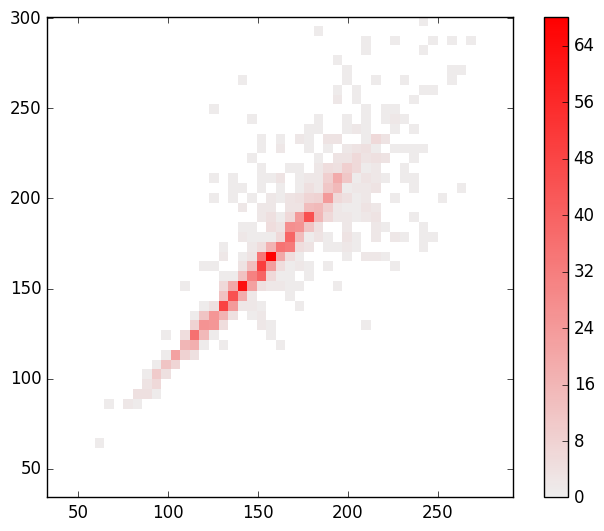
\includegraphics[scale=0.4]{img_size/lamellarity/heatmap_multilamellar.png} & 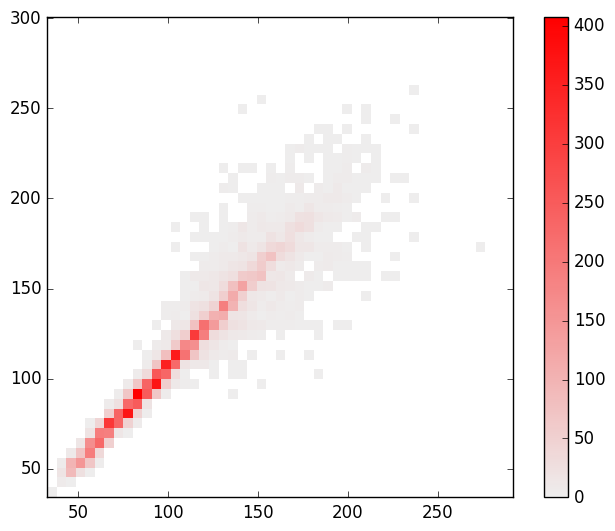
\includegraphics[scale=0.4]{img_size/lamellarity/heatmap_unilamellar.png} & 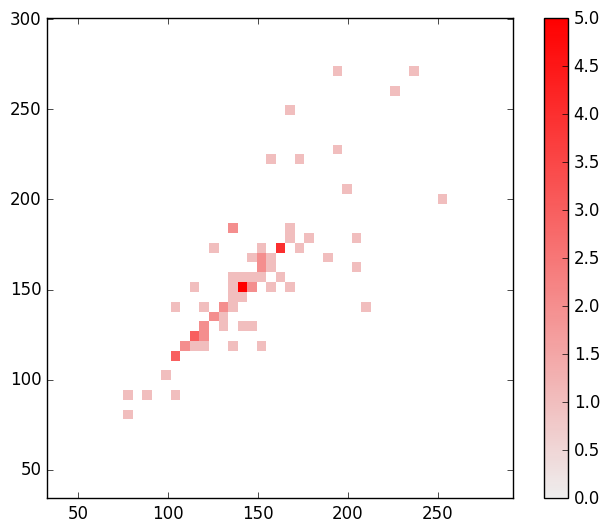
\includegraphics[scale=0.4]{img_size/lamellarity/heatmap_uncertain.png} \\
	Multilamellar & Unilamellar & Uncertain \\[6pt]
	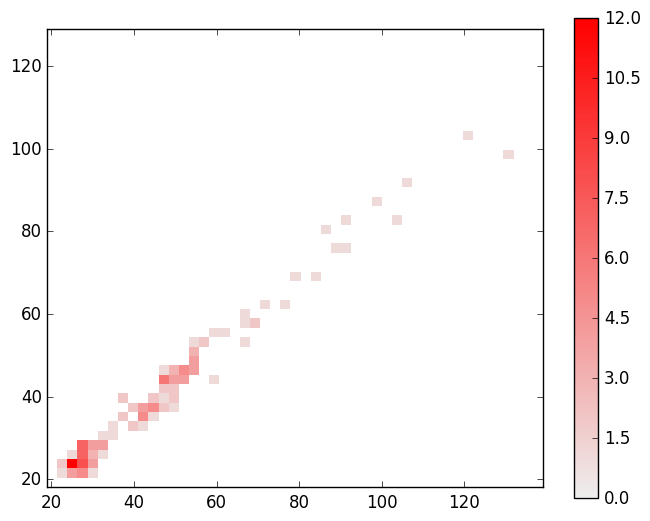
\includegraphics[scale=0.4]{img_size/encapsulation/heatmap_empty.png} & 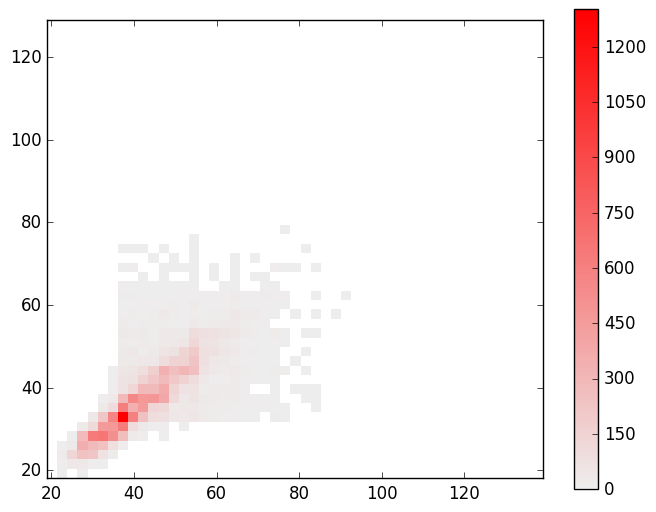
\includegraphics[scale=0.4]{img_size/encapsulation/heatmap_full.png} & 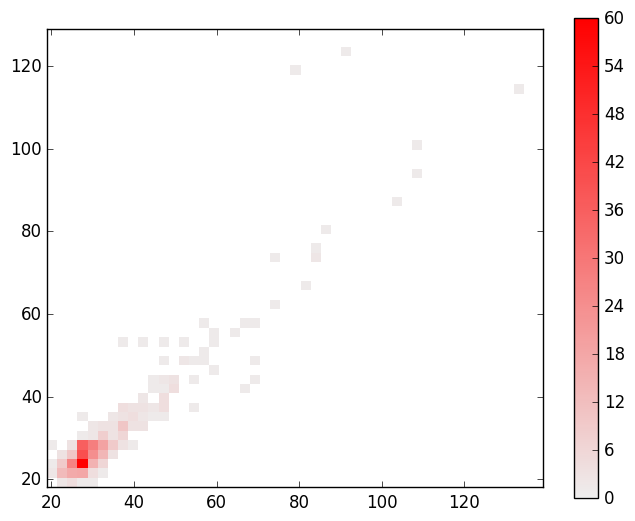
\includegraphics[scale=0.4]{img_size/encapsulation/heatmap_uncertain.png} \\
	Empty & Full & Uncertain \\[6pt]
\end{tabular}
\caption{Distribution of image sizes in each class. The upper row corresponds to the lamellarity problem, the lower corresponds to the encapsulation problem.}
\label{fig:img_size_per_class}
\end{figure}
\end{landscape}


\section{Methodology}

\subsection{Support Vector Machines}
\label{sec:svm}
The support vector machine (SVM) is one of the most influential approaches to supervised learning~\cite{Boser:1992:TAO:130385.130401}. SVM is driven by a linear function $w^\top x + b$~\cite{dl_book}. In the classification tasks, SVM has the aim to determine decision boundaries that produce optimal class separation. SVM was initially designed for binary classification cases but a number of modifications were introduced for multiclass classification. One of them is the "one-against-one" approach~\cite{Knerr1990}. According to this technique, $n (n-1)\frac{1}{2}$ classifiers are trained for each class, where $n$ is the number of classes. SVM does not provide probabilities, just a class identity~\cite{dl_book}. The \texttt{LIBSVM}~\cite{CC01a} library is used for experiments in this project and it implements the "one-against-one" technique.

Currently automatic classification is performed by means of SVM at Vironova. The performance of the SVM classifier has shown up to $98\%$ accuracy on the lamellarity problem and up to $87\%$ on the encapsulation problem. The following object features are used by Vironova:
\begin{itemize}
\item Area
\item Circularity
\item Image moments $\mu_{20}$, $\mu_{02}$, $\mu_{30}$, $\mu_{03}$
\item Edge density profile
\item Histogram
\item Internal segmentation variance
\end{itemize}

All named above features except internal segmentation variance are described in section~\ref{sec:dataset}. Internal segmentation variance is not available in provided data sets but its absence had insignificant impact on experiment results as shown later in this report.  

\subsection{Convolutional Neural Networks}
Convolutional networks~\cite{LeCun1986}, also known as convolutional neural networks or CNNs, are defined in~\cite{dl_book} as: \blockquote{specialized kind of neural network for processing data that has a known, grid-like topology. Convolutional networks are simply neural networks that use convolution in place of general matrix multiplication in at least one of their layers.}

Employing CNNs for this project as the main tool for performing classification tasks is motivated in the following way. Since the introduction in~\cite{LeCun1986} in the late 1980's, CNNs have demonstrated excellent performance in object detection and recognition tasks. One of the most influential applications of CNNs is in the ImageNet 2012 competition that was won using a CNN model~\cite{NIPS2012_4824} with an error rate of $16.4\%$ which was a breakthrough at that time. There are also examples of successful applications of CNNs in the microscopy image domain. For example U-Net~\cite{Ronneberger2015} has solved a biomedical image segmentation task although provided with very limited training data. The area of CNN applications is extensive and they are being used by all leading IT companies such as Google, Facebook, Microsoft and others. The current interest for CNNs is driven mainly by three factors~\cite{Zeiler2014}: the availability of large annotated data sets, powerful GPU hardware, and better model regularization strategies. 

CNNs are of great interest in the image analysis domain because they allow learning of image features. One does not need to be an image analysis specialist to build a powerful and robust image classification or object recognition system. Unlike many other methods in image analysis, CNNs do not require handcrafted characteristic features designed by an image analysis specialist, even though these features can be incorporated in a CNN model. For instance, the lamellarity and encapsulation problems have already been successfully solved by Vironova specialists using the SVM combined with carefully selected object features such as area, circularity, image moments and the other features discussed in section~\ref{sec:svm}. This project studies the CNNs ability to achieve comparable result without using handcrafted features.

\subsection{Architecture Overview}

A CNN can be configured according to a wide variety of architectures. There is no general rule that says how to configure a CNN for a specific task but there are some best practices and general recommendations. Probably the most influential CNN architectures are VGG~\cite{DBLP:journals/corr/SimonyanZ14a}, AlexNet~\cite{NIPS2012_4824} and GoogleNet~\cite{DBLP:journals/corr/SzegedyLJSRAEVR14}.

According to~\cite{dl_book} a typical building block of a convolutional neural network consists of three stages:
\begin{enumerate}
\item \textbf{Convolutions}. The convolutional layer is the core building block of a CNN. Here most of the computations are done. The convolutional layer's parameters are a set of learnable filters. A filter is usually small spatially, i.e. along width and height, and extends through the full depth of the input volume. For example, if an input image to some CNN has three color channels, then the filter on the first layer will have size $n \times n \times 3$, where $n$ if some small integer. If we decide to apply 32 such filters on the first convolutional layer the then filters on the second one will have size $n \times n \times 32$. 

Convolutions can be made with filters of different sizes, different padding strategies and stride values. The stride value specifies how many pixels is the filter is moved at a time. Different padding modes affect the size of the output. The most common strategies are \textit{valid} and \textit{same}. \textit{Valid}, Figure~\ref{fig:padding_valid}, implies that the convolution is performed only at those positions were the filter is within the image bounds. This results in a reduced size of the layer output compared to the layer input. \textit{Same}, Figure~\ref{fig:padding_same}, implies zero padding in order to preserve the input size.  

There are two very important assumptions about the convolutional layers: local connectivity and parameters sharing. Local connectivity implies that each neuron of the convolutional layer is not connected to all neurons on the previous one, but only to a subregion of the previous layer. Parameter sharing implies that all neurons of the convolutional layer have the same weights. These two assumptions are illustrated in details in Figure~\ref{fig:local_connectivity}.	

\item \textbf{Nonlinearity}. At this stage, the linear activations produced on the previous step are run through some nonlinear activation function. One of the most widely used is ReLU which is defined as $f(x) = max(0, x)$.
 
\item \textbf{Pooling}. This is used to modify the output of the layer further. A pooling function replaces the output of a layer at certain positions with a summary statistic of the surrounding region. The size of this region is subject of a design decision. In practice, $2 \times 2$ pooling is often used. The most popular summary statistics is $max$, however others, such as average, are also possible. Pooling is usually followed by dropout for regularization purposes. Dropout is discussed in details in section~\ref{sec:dropout}. Springenberg et al. shows in~\cite{DBLP:journals/corr/SpringenbergDBR14} that max-pooling layers can successfully be replaced with convolutional layers with corresponding stride values. 
\end{enumerate}

A frequent source of confusion is the dimensionality of the convolutional layer output. Let us discuss it in more details. Recall that an image is usually represented as a 3 dimensional array, where first two dimensions correspond to width and height while the third one corresponds to the number of color channels. The number of color channels is 1 for grayscale images, 3 for RGB images, etc. Let us call the third dimension as depth. Note that "depth" does not correspond to the number of layers in the CNN in this context. Convolutional layer output is also three-dimensional. Width and height are controlled by  such parameters as filter size, stride and padding mode. The third one, which is depth, is also controlled by a parameter, that corresponds to the number of filters we would like to use.

For example, if a convolutional network takes as input the raw grayscale $32 \times 32$ image and uses 32 $3 \times 3$ filters on the first layer with unit stride and \textit{valid} padding, then the output of the first layer would be of size $30 \times 30 \times 32$. Technically speaking, input and output to the CNN is four-dimensional, where the first dimension is the batch size, i.e. the number of images being processed. Here it was omitted for the sake of simplicity. Note that I put depth dimension at the end, but it is really a matter of convention. Different software tools employ different conventions, so it is not uncommon to see the depth dimension on the second place, like $[b, d, w, h]$ where $b$ is the batch size, $d$ is depth, $w$ is width and $h$ is height. 

Dimensionality in the depth dimension can be either reduces or increased on purpose. Sometimes it is desirable to decrease the number of depth dimensions before some computationally expensive operations. The tool that allows this is so called $1 \times 1$ convolution. For example, authors of~\cite{DBLP:journals/corr/SzegedyLJSRAEVR14} use   $1 \times 1$ to reduce dimensionality in the depth dimension before the expensive $3 \times 3$ and $5 \times 5$ convolutions. Note that $1 \times 1$ convolutions affect only the depth, they leave spatial dimensions (width and height) unaffected.

Usually a number of convolutional layers is combined with a number of fully connected layers at the end. In such case the output of the last convolutional layer is flattened, i.e. collapsed into one dimension, and a number of fully connected layers goes  to the final layer. The final layer has softmax activation and a number of nodes that is equal to the number of classes. Such  approach is simple and is efficiently implemented in many software tools but it has one important constraint. It requires input of a fixed size. Such networks can not handle images of different sizes. If it is required to build a model that can process images of arbitrary size then a fully convolutional neural network (FCNN) is a possible solution. A FCNN does not require the input to have fixed size and can be trained on images of variable size. Fully convolutional in this context means that the network does not have any fully connected layers, only convolutional. FCNNs have proven to be especially effective in semantic segmentation tasks~\cite{DBLP:journals/corr/ShelhamerLD16}.

Figure~\ref{fig:conv_net} summarizes all mentioned above statements and gives an example of the CNN workflow.  

\begin{figure}[H]
\centering
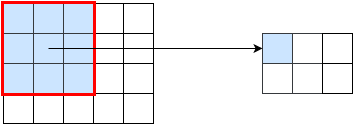
\includegraphics[scale=0.7]{padding_valid.png} 
\caption{Illustration of the \textit{valid} padding mode. Assume that a $3 \times 3 \times 1$ (a red frame) convolutional filter is applied to a $5 \times 5 \times 1$ input volume (to the right). Result of the convolution is to the left. The \textit{valid} mode implies that convolution is performed only at those positions when it fully fits into the input volume, these results in reduced size of the output compared to the input.}
\label{fig:padding_valid}
\end{figure}

\begin{figure}[H]
\centering
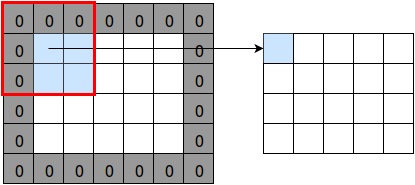
\includegraphics[scale=0.7]{padding_same.png} 
\caption{Illustration of the \textit{same} padding mode. Assume that a $3 \times 3 \times 1$ (a red frame) convolutional filter is applied to a $5 \times 5 \times 1$ input volume (to the right). Result of the convolution is to the left. The \textit{same} padding mode implies adding zero padding to the input of the size which is enough to make the output of the same size as the input, which is $\frac{n-1}{2}$, where $n$ is the size of the filter.} 
\label{fig:padding_same}
\end{figure}

\begin{figure}[H]
\centering
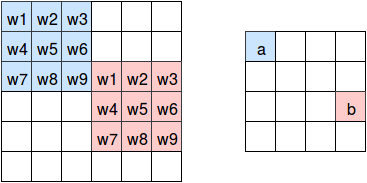
\includegraphics[scale=0.7]{local_connectivity_parameter_sharing.png} 
\caption{Illustration of local connectivity and parameter sharing (best viewed in color). Matrix on the left is input to the convolutional layer on the right. Here we assume \textit{valid} padding mode and filter size of 3. Each neuron of the convolutional layer is connected only to a small subregion of the input. The size of the subregion corresponds to the size of the convolutional filter. For example, neuron $a$, highlighted in blue, is connected to 9 inputs in the upper-left corner, neuron $b$ is also connected to only 9 inputs out of 36. Moreover, all neurons in the convolutional layer share their weights, so neurons $a$ and $b$ have the same weights $w_i$, $i \in [1, 9]$. These two assumptions reduce number of parameters drastically. If all neurons in this example where fully connected this would result in $16 * 36 = 576$ parameters. But with local connectivity and parameter sharing the number of unique weights is only 9. Note that weights are shared only across spatial dimensions of the filter, they are still unique across the depth dimension. If the filter size was $3 \times 3 \times 3$, there would be 27 unique parameters.}
\label{fig:local_connectivity}
\end{figure}

\begin{landscape}
\begin{figure}[H]
\centering
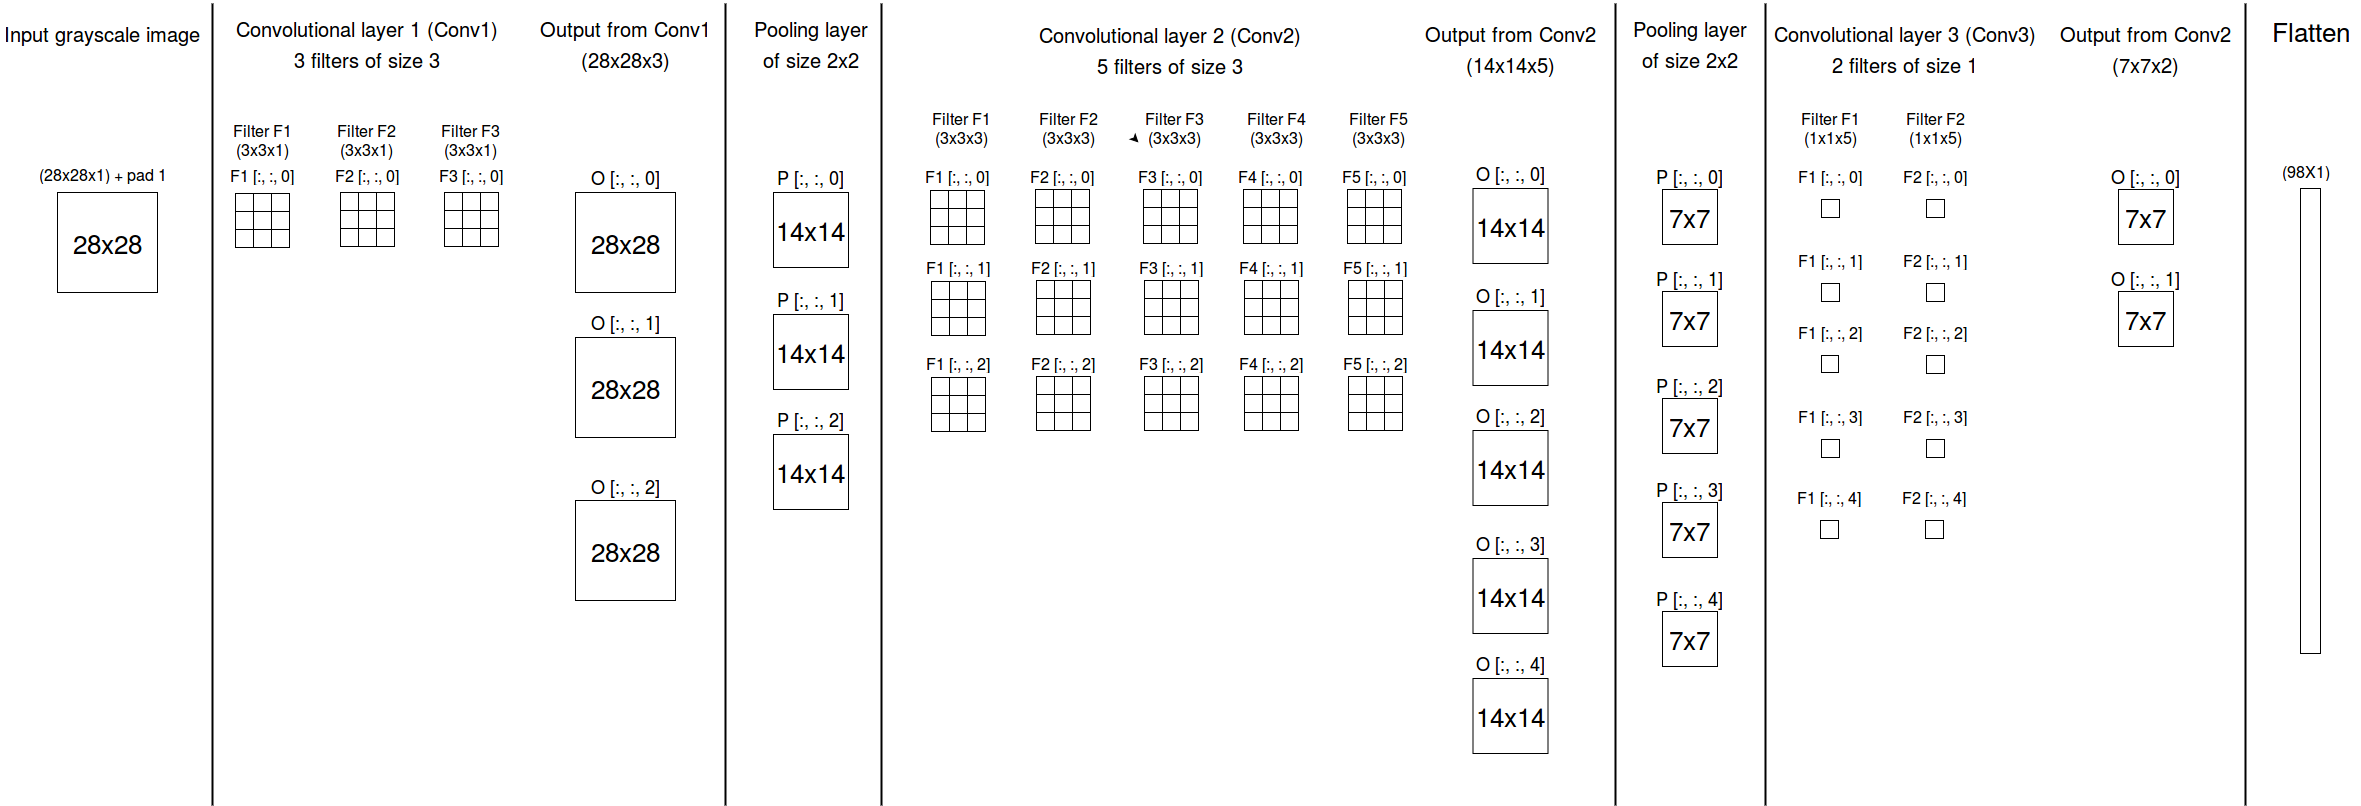
\includegraphics[width=\linewidth]{conv_net.png} 
\caption{An example of the CNN workflow. Here we assume grayscale $28 \times 28$ input image, \textit{same} padding mode and unit stride for all convolutional layers. The first convolutional layer consists of three $3 \times 3 \times 1$ filters, so its output is of size $28 \times 28 \times 3$. On the next layer max-pooling operation of size 2 is applied. This affects spatial dimensions, but not the depth. This layer yields output of size $14 \times 14 \times 3$. The third layer is convolutional and here 5 filters of size $3 \times 3 \times 3$ each are applied. The output has size $14 \times 14 \times 5$. Input image is convolved with each filter and summed across all depth dimensions. For example, output $O[:, :, 0]$ is the sum of convolving inputs $P[:, :, i]$ with filters $F_1[:, :, i]$, where $i \in [0, 1, 2]$. The fourth layer is max-pooling of size 2 so its input is $7 \times 7 \times 5$. Lets us demonstrate depth dimension reduction with the final convolutional layer which consists of two $1 \times 1 \times 5$ filters. This layer yields $7 \times 7 \times 2$ input. Note that spatial size is unaffected while number of depth dimensions is reduced from five to two. The last layer on this illustration is flattening operation which collapses $7 \times 7 \times 2$ volume into a vector of length $98$. After flattening a number of fully connected layers can be applied. Note that activation layers have been omitted on this illustration. Usually, some non-linearity, like for example ReLU, is applied to the output of the convolutional and fully-connected layers.}
\label{fig:conv_net}
\end{figure}
\end{landscape} 


\subsection{Deconvolutional Neural Networks}
Convolutional neural networks is a powerful machine learning method that is capable of learning the image features in order to describe provided categories. However, it is usually not obvious what kind of features the model has learned. For some time convolutional neural networks have been treated as a black box. This changed in 2014 when Zeiler et al.~\cite{Zeiler2014} proposed \textit{Deconvolutional Networks (DN)} for visualization of convolutional  neural networks, or rather patterns that fire network activations. In this way it is much easier to understand how convolutional neural networks \blockquote{see} images. 

The DN method can be summarized in the following way. The deconvolutional network goes down from activations of a given layer back to the image. In this manner DN reverses data flow of a CNN undoing the effect of convolutions. The resulting reconstructed image shows parts of the input image that caused the strongest activations. 

In order to reverse the data flow of a CNN, all its components must be reversible. To invert learned, filters DN transposes them which means in practice flipping each filter vertically and horizontally. CNN usually use rectifiers as activation functions that guarantee that feature maps are always positive. Features are reconstructed using the same ReLU non-linearities. Pooling is a common building block of any CNN. Unlike convolution and rectification pooling generally can not be undone, it is not reversible. Zeiler et al. proposed to record the locations of the maxima within each pooling region, they call these recorded values switch variables. The unpooling operation uses switches to place reconstructions into appropriate locations, setting other values within the upsampling region to zero.

Convolutional networks that replace the max pooling operation with convolution with stride can be visualized in a similar way. Springenberg et al.~\cite{DBLP:journals/corr/SpringenbergDBR14} propose modifications to the DN method that achieve similar results as in~\cite{Zeiler2014}.

\subsection{Optimization}
Deep learning algorithms involve optimization in many contexts~\cite{dl_book}. The most obvious one is finding network parameters that reduce a cost function. One design decision that has to be made is the choice of optimization method. In this project I limited the choice of optimizers to ADAM~\cite{DBLP:journals/corr/KingmaB14} and Stochastic Gradient Descent (SGD)~\cite{Zhang04solvinglarge}. 

Stochastic gradient descent is a stochastic approximatoin of the gradient descent optimization method for minimizing an objective function. SGD combined with the backpropagation algorithm is the most common method for training artificial neural networks~\cite{LeCun1998}.

ADAM (Adaptive Moment Estimation) is a novel optimization method which brings some important modifications to the SGD algorithm. ADAM's update rule uses both the average of past stored gradients and the average of past squared gradients. Both average values are exponentially decaying. 

\subsection{Performance measures}

When evaluating a classification model, one is almost always interested in how many predictions from all predictions made that are correct. In other words we are interested in how accurate a particular model is. The accuracy of a classification system is the share of correct predictions of the total number of examples. Accuracy  is one of the most frequently used performance measures in classification problems. However accuracy alone is usually not enough to describe the predictive power of the model. Models with a given accuracy may have greater predictive power than models with higher accuracy. This is known as the Accuracy Paradox~\cite{zhu2007knowledge}.

Let's illustrate the Accuracy Paradox using the encapsulation problem. Table~\ref{table:encapsulation_dataset} on page~\pageref{table:encapsulation_dataset} presents the distribution of the three classes in the encapsulation data set. Consider a model that classifies all particles as full. Such a model would achieve the astonishing accuracy of $97\%$ just by making the same prediction for all particles. Let's compare it to another model, that makes a random guess, i.e. predicts each class with $\frac{1}{3}$ probability. Such a random guess model would have an accuracy of approximately $33\%$, almost three times less than the first model. However, while the first model totally ignores two minority classes, the second one has $33\%$ chance of detecting them, so it may be preferred comparing to the first one. 

Imbalanced data sets is a typical reason to when accuracy is misleading and fails as a performance measure. An unambiguous way to present the prediction results of a classification model is a confusion matrix~\cite{STEHMAN199777}. A confusion matrix is a table with the number of rows and columns both equal to the number of classes in the data set under consideration. Columns represent predicted classes and rows represent true classes. Each cell contains the number of predictions that corresponds to that particular category. 

A table of confusion is a special case of confusion matrix that deals with binary classification. A table of confusion is presented in Table~\ref{table:table_of_confusion} and it is usually used to illustrate performance measures that are derived from a confusion matrix.

\begin{center}
\captionof{table}{Table of confusion}
\label{table:table_of_confusion}
\begin{tabular}{|c|c|c|}
\hline 
 & Predicted True & Predicted False \\ 
\hline 
Actual True & \specialcell{True positive \\ TP} & \specialcell{False negative \\ FN} \\ 
\hline 
Actual False & \specialcell{False positive \\ FP} & \specialcell{True negative \\ TN} \\ 
\hline 
\end{tabular} 
\end{center}
 
Different performance measures are discussed and compared in~\cite{powers07evaluation}. The rest of this section presents performance measures that are used in this project for evaluation and comparison of different classification models. 

\textbf{True positive rate (TPR)}, also known as sensitivity or recall, measures the share of positives that have been correctly identified:
\begin{equation*}
TPR = \frac{TP}{TP + FN}
\end{equation*}

\textbf{True negative rate (TNR)}, also known as specificity, measures the share of negatives that have been correctly identified:
\begin{equation*}
TNR = \frac{TN}{TN + FP}
\end{equation*}

\textbf{Positive predicted value (PPV)}, also known as precision, measures the share of correct positive predictions:
\begin{equation*}
PPV = \frac{TP}{TP + FP}
\end{equation*}

\textbf{Negative predicted value (NPV)} measures the share of correct negative predictions:
\begin{equation*}
NPV = \frac{TN}{TN + FN}
\end{equation*}

The $F_1$ score is a harmonic mean of TPR and TNR, which is a measure of a test's accuracy. It reaches its best value at 1 and worst at 0. 
\begin{equation*}
F_1 = \frac{2}{\frac{1}{TPR} + \frac{1}{TNR}}
\end{equation*}
$F_1$ has been criticized for not taking true negatives into account and a number of alternative measures such as Phi coefficient, Matthews correlation coefficient and Cohen's kappa have been proposed~\cite{powers07evaluation}. However, let us use $F_1$ anyway for the sake of simplicity.   

Combining all measures presented above allows more detailed analysis of the classifier performance. 

\subsection{Loss function}
\label{sec:loss_function}
This section is taken from~\cite{mlprojectreport}.

The multi-class logarithmic loss function is a loss function that represents the price paid for inaccuracy of predictions in classification problems~\cite{rosasco}. The formula is:
\begin{equation}
loss = -\frac{1}{N} \sum_{i=1}^{N} \sum_{j=1}^{M} y_{i,j} log(p_{i,j})
\end{equation}

Where 
\begin{itemize}
\item N -- number of observations
\item M -- number of classes, it is three in our case
\item \textit{log} -- natural logarithm
\item $y_{i,j}$ -- is 1 if observation $i$ is in class $j$ and 0 otherwise
\item $p_{i,j}$ --  is the predicted probability that observation $i$ is in class $j$
\end{itemize}

In order to calculate multi-class logarithmic loss, the classifier must assign a probability to each class rather than simply yielding the most likely class. This fact constitutes the main difference between accuracy and logarithmic loss. In order to consider a prediction as accurate, it is sufficient that the classifier marks the correct class as the most likely one, no matter how confident the prediction is.

Figure~\ref{fig:logloss} shows log loss from a single class where predicted probability ranges from 0 (the completely wrong prediction) to 1 (the correct prediction). As predicted probability moves closer to 1, log loss decreases gently to 0. On the contrary, log loss increases rapidly as predicted probability moves towards zero. It is clear from Figure~\ref{fig:logloss} that the multi-class logarithmic loss heavily penalizes classifiers that are confident about an incorrect classification.

\begin{figure}[H]
\centering
\begin{tikzpicture}
\begin{axis}[
	axis lines = left,
	xlabel = Predicted probability,
	ylabel = Loss,
]
\addplot [
	domain=0.0001:1,
	samples=100,
	color=red,
]
{-ln(x)};
\addlegendentry{$f(x) = -log(x)$}
\end{axis}
\end{tikzpicture}
\caption{\label{fig:logloss} Log loss of a single class where predicted probability ranges from 0 to 1. }
\end{figure}

Consider an example of a binary classifier and let us take a look at the effect of various predictions for class membership probability. 
\begin{itemize}
\item Classification that assigns equal probabilities to both classes results in loss $-log(0.5)=0.6932$.  

\item Classification confident in the correct class results in loss $-log(0.9)=0.1054$.

\item Classification confident in the wrong class results in loss $-log(0.1)=2.3026$. 
\end{itemize}

In other words, the log loss function encourages moderate predictions. It is better to make all classifications neutral rather than make 50\% correct classifications and 50\% completely wrong predictions.

\subsection{Class Imbalance Problem}
\label{sec:class_imbalance}
The encyclopedia of Machine Learning~\cite{Ling2010} defines the Class Imbalance problem as follows:
\blockquote{Data are said to suffer the \textit{Class Imbalance Problem} when the class distributions are highly imbalanced. In this context, many classification learning algorithms have low predictive accuracy for the infrequent class.}

It is a serious problem because most machine learning algorithms will tend to classify all examples as the majority class and to treat examples of minority class as noise. The lamellarity and encapsulation data sets presented in section~\ref{sec:problem_description} are highly imbalanced. In the lamellarity data set, the majority class accounts for $87\%$ of all samples and in the encapsulation data set, the majority class constitutes $97\%$ of all samples. Preliminary experiments showed that classifiers trained on raw unbalanced data sets are highly biased towards the majority classes and do not generalize well. However the class imbalance problem is not uncommon. In fact, data sets are highly imbalanced in many domains, for example fraud detection, medical diagnosis, anomaly detection, telecommunications, etc. 

Various solutions have been proposed to deal with this problem and they can be summarized into three groups~\cite{Lopez2013113}:

\begin{itemize}

\item \textit{Data sampling} implies any means to produce a more or less balanced data set. It can for example be oversampling, undersampling, SMOTE (Synthetic Minority Over-sampling Technique)~\cite{smote_chawla} or generating artificial examples~\cite{ishaq_synthetic}. The data sampling method usually performs best combined with data augmentation techniques.

\item \textit{Algorithm modification} is oriented towards the adaptation of base learning methods to be more attuned to class imbalance issues~\cite{Zadrozny:2001:LMD:502512.502540}.

\item \textit{Cost sensitive learning} introduces higher penalties for misclassification of minority classes making learning algorithm more sensitive to underrepresented classes. 

\end{itemize}

The methods listed above prevent classifiers from ignoring underrepresented classes during the training phase. However this is very likely to lead to another problem --- overfitting. Overfitting is discussed in section~\ref{sec:regularization}. The rest of this section discusses methods that have been used to mitigate the Class Imbalance Problem in the lamellarity and encapsulation data sets. 


\subsubsection{Oversampling}
Oversampling means repeating instances of underrepresented classes. Minority classes in the lamellarity data set are the multilamellar and uncertain, and in the encapsulation data set --- empty and uncertain. Examples of these classes are repeated to match the number of majority class samples so that training sets become balanced. Oversampling itself does not mitigate the imbalance problem much, it works best combined with data augmentation which is discussed in section~\ref{sec:data_augmentation}.

\subsubsection{Undersampling}
Undersampling, as opposed to oversampling, means excluding some samples of the majority class in order to make the training set balanced. In practice, undersampling is repeated at the beginning of each learning epoch when randomly selected samples are excluded. In such a way the learning algorithm can still use all samples for training, it just does not see all of them during all epochs. The proportion of excluded samples can vary and depends on the context. In the experiments presented in this project, undersampling implies dropping $20\%$ of the majority class samples. 

\subsubsection{SMOTE}
Synthetic Minority Over-sampling Technique (SMOTE) is an over-sampling approach in which the minority class is over-sampled by creating “synthetic” examples rather than by over-sampling with replacement~\cite{smote_chawla}. 
Synthetic examples are generated by combining each minority class example with its randomly selected $k$ nearest neighbors in feature space, where $k$ is a parameter that depends on amount of required over-sampling. Selection of feature is a design decision and varies between different problems.

\subsubsection{Artificial data}
Machine learning algorithms perform best when provided with large training data sets. In many domains, including medicine and biology, expert annotation is required for preparing training and test data sets. This results in high cost and effort, so the size of data sets is often limited. In such a case artificial data is an attractive alternative to real expert-annotated data. Training of convolutional neural network models for fluorescent spot detection on artificial data is e.g., discussed and evaluated in~\cite{ishaq_synthetic}. 

\begin{figure}[H]
\centering
\begin{tabular}{ccc}
	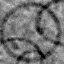
\includegraphics[scale=1.5]{synthetic/uni.png} & 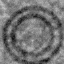
\includegraphics[scale=1.5]{synthetic/multi.png} & 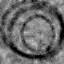
\includegraphics[scale=1.5]{synthetic/uncertain.png} \\
	Unilamellar & Multilamellar & Uncertain \\[6pt]
\end{tabular}
\caption{Artificial examples for lamellarity problem}
\label{fig:synthetic_images}
\end{figure}

In this project artificial data has been generated for the lamellarity problem. Artificial images of liposomes are generated by drawing circles with carefully selected randomized distortions. Background and distortions are generated using Perlin noise~\cite{Perlin:1985:IS:325165.325247}. Perlin noise was selected because of visual similarity of its output to the actual EM images. Figure~\ref{fig:synthetic_images} presents examples of artificially generated EM images. These artificial examples contain random shift transformation so they are not centered as the real examples in Figure~\ref{fig:lamellarity_problem}.

Note that despite visual similarity, artificial images are not based on statistical measures from the real data set. Histograms and image patterns are not drawn from real distributions. With limited time and effort, this experiment should be rather seen as a proof of concept.

\section{Regularization}
\label{sec:regularization}

Let us assume that an imbalanced data set has been balanced by a combination of the methods described in section~\ref{sec:class_imbalance}. This would significantly reduce the training error which means that the model is able to describe the data generation process of the training set. 

However as the result of seeing multiple copies of the minority classes, the learning algorithm will almost certainly describe random error or noise as well. Such a model would not be able to make reliable predictions on general untrained data, i.~e. its generalization error would be unacceptably high. As defined in~\cite{dl_book}, \blockquote{\textit{Regularization} is any modification we make to a learning algorithm that is intended to reduce its generalization error but not its training error}.

The rest of this section presents regularization techniques that have been used to reduce generalization error of models trained on the lamellarity and encapsulation data sets.

\subsection{Weight decay}
Weight decay is a method of adding a penalty to the weight magnitudes of the hidden layer to the loss function. In this way we express preference of smaller weights and prevent weight of some hidden nodes or convolutional filters from becoming too large. Large weights can result in undesired numerical errors such as overflow or truncation error. Usually the $L^2$ norm of penalized layers multiplied by some constant $\alpha$ (typically close to zero) is added to the loss function. However other norms such, as but not limited to, $L^1$ can be used. 
On the other hand, weight decay can lead to other problems as described in~\cite{dl_book}. Penalties on weights can cause non-convex optimization procedures to get stuck in local minima corresponding to small values of weights. 

Applied to neural networks it means that weight decay can lead to \blockquote{dead units}. These units do not contribute much to the learning process because their input and output weights are all very small. This configuration can be locally optimal even if loss value can be significantly reduced by making the wights larger. This phenomenon was observed during the experiments presented in this project. Applying weight decay to convolutional layers resulted in numerous dead filters which worsened the classifier's performance on both training and test sets.

\subsection{Noise injection}
Noise robustness can be achieved by adding some noise to the model. Noise can be added at several places. 

Firstly, noise can be added to the input data, in our case to EM images. 

Secondly, noise can be added to weights. This technique is primarily used in recurrent neural networks~\cite{pmid18263536}. 

Thirdly, most data sets have some mistakes in the annotated labels. As shown in section~\ref{sec:loss_function}, it can be very costly to maximize $\log p(y|x)$ when label $y$ is wrong. Label smoothing technique is proposed in~\cite{dl_book}. A label smoothing regularizes a model based on a softmax with $k$ output values by replacing the hard 0 and 1 classification targets with targets of $\frac{\epsilon}{k}$ and $1 - \frac{k-1}{k}\epsilon$, respectively, where $\epsilon$ is an arbitrary value between 0 and 1, usually very close to 0. The label smoothing operation can be written as~\ref{eq:soft_targets}.

\begin{equation}
\label{eq:soft_targets}
x \leftarrow x \left( 1 - \epsilon \right) + \left(1 - x\right) \frac{\epsilon}{k - 1}
\end{equation}

Label smoothing is used in all experiments presented in this project.

\subsection{Dropout}
\label{sec:dropout}
Dropout~\cite{JMLR:v15:srivastava14a} suggests to randomly drop non--output units (nodes) along with their connections from the network. This prevents units from co--adapting too much. Dropout is implemented as a parameter between $0$ and $1$ that describes the probability of dropping each unit. It can be constant during all training epochs or some decay scheme may be used. Dropout may be more aggressive in the beginning of the training and smaller later when the model becomes trained. It is the same idea as with learning rate decay. Dropout is used in all experiments presented in this project.


\subsection{Early stopping}
Early stopping is probably the most commonly used regularization strategy in deep learning~\cite{dl_book}. It is a simple yet powerful technique of determining the optimal number of training epochs. <the idea is to split the training data into a train set used to train the model and a validation set, which is not used in the training process. Errors of both sets are monitored at each epoch. Training should be stopped when the validation set performance has not improved for some selected number of epochs. This prevents overfitting and improves generalization. Validation set error is more suitable than training set error because training error decreases steadily over time as the model starts to overfit while validation error begins to rise again. 
In this project early stopping is used to determine the number of training epochs, that is later fixed during k-fold cross validation.

\subsection{Data augmentation}
\label{sec:data_augmentation}
As was already mentioned in section~\ref{sec:class_imbalance}, training data is often limited and additional data is hard to obtain. One way to get around this problem is to introduce additional diversity in the training set by augmenting existing data. Data augmentation has proven to be especially effective for classification tasks~\cite{dl_book} which is exactly the case in this project. 
A good classifier is invariant to a wide variety of transformations and can see the true class from \blockquote{different points of view}. New $(x, y)$ pairs, where $x$ is a class example and $y$ is corresponding label, can be easily generated by applying different transformations to $x$. The choice of transformations is highly application dependent. For example, optical recognition models must recognize the difference between `b' and `d' and between `6' and `9', so horizontal and vertical flips are not suitable for this task. 
 
In this project, data is augmented in the following way:

\begin{itemize}
\item Rotation in the range $[-180, 180]$ degrees with spline interpolation
\item Shear transformation in the range $[0, 0.2]$
\item Vertical shift in the range $[-10, 10]$ percent of total height
\item Horizontal shift in the range $[-10, 10]$ percent of total width
\item Zoom in the range $[0.8, 1.0]$ which means zoom by a maximum $20\%$
\item Horizontal flip
\item Vertical flip
\end{itemize}

All transformations are applied randomly. Horizontal and vertical flips are performed with $50\%$ probability, rotation, shear, shift and zoom values are uniform random integer values in specified ranges. Data augmentation is performed in all experiments unless the opposite is stated explicitly.

Figure~\ref{fig:augmented_images} show an example of data augmentation. Thus a model never sees two identical examples during training.

\begin{figure}[H]
\centering
\begin{tabular}{ccccc}
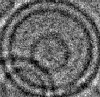
\includegraphics[scale=0.5]{augmented/541253.jpg} & 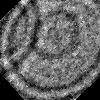
\includegraphics[scale=0.5]{augmented/_0_645.jpeg} & 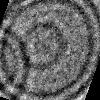
\includegraphics[scale=0.5]{augmented/_0_1385.jpeg} & 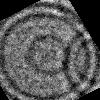
\includegraphics[scale=0.5]{augmented/_0_1749.jpeg} & 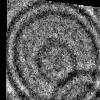
\includegraphics[scale=0.5]{augmented/_0_2343.jpeg} \\

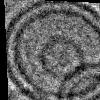
\includegraphics[scale=0.5]{augmented/_0_4050.jpeg} & 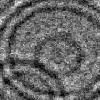
\includegraphics[scale=0.5]{augmented/_0_3413.jpeg} & 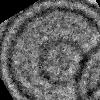
\includegraphics[scale=0.5]{augmented/_0_3414.jpeg} & 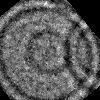
\includegraphics[scale=0.5]{augmented/_0_3687.jpeg} & 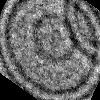
\includegraphics[scale=0.5]{augmented/_0_3916.jpeg} \\
	
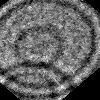
\includegraphics[scale=0.5]{augmented/_0_4165.jpeg} & 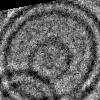
\includegraphics[scale=0.5]{augmented/_0_5014.jpeg} & 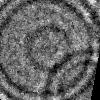
\includegraphics[scale=0.5]{augmented/_0_5165.jpeg} & 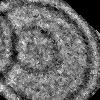
\includegraphics[scale=0.5]{augmented/_0_5567.jpeg} & 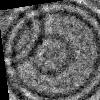
\includegraphics[scale=0.5]{augmented/_0_6089.jpeg} \\

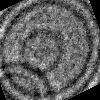
\includegraphics[scale=0.5]{augmented/_0_7140.jpeg} & 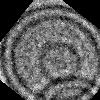
\includegraphics[scale=0.5]{augmented/_0_7746.jpeg} & 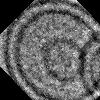
\includegraphics[scale=0.5]{augmented/_0_8553.jpeg} & 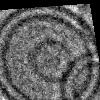
\includegraphics[scale=0.5]{augmented/_0_8763.jpeg} & 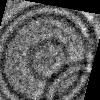
\includegraphics[scale=0.5]{augmented/_0_9361.jpeg} 
	
\end{tabular}
\caption{Examples of data augmentation. The upper left is an original image and all other images are the results of random transformations described in this section.}
\label{fig:augmented_images}
\end{figure}

\section{Review of deep learning software tools}

A wide variety of deep learning software tools is available to the public. Most of them are open-source and are distributed under licenses that allow commercial use. Development of deep learning frameworks is driven by Universities and leading IT companies such as Google and Microsoft with extensive help from the community. For example Theano~\cite{2016arXiv160502688short} at the University of Montreal is one of the first and most influential deep learning libraries. It was initially released in 2010. Another state of the art tool is Caffe~\cite{jia2014caffe} by UC Berkeley. Google released the TensorFlow~\cite{tensorflow2015-whitepaper} software library in November 2015. Microsoft made its CNTK~\cite{cntk} tool available to the public in January 2016.

The above mentioned software tools together with some other are summarized in Table~\ref{tbl:comparison_of_dl_lib}. 

Four deep learning libraries: TensorFlow, Caffe, Torch~\cite{Collobert_NIPSWORKSHOP_2011} and CNTK have been compared and benchmarked in~\cite{DBLP:journals/corr/ShiWXC16}. Authors have concluded that \blockquote{all tested tools can make good use of GPUs to achieve significant speedup over their CPU counterparts. However, there is  no  single  software  tool  that  can  consistently  outperform other.} Their tests of CNN models showed that Caffe and Tensorflow performed best on CPUs with 4 and 16 threads respectively. On GPU, Caffe, Tensorflow and CNTK were best depending on mini-batch size and GPU type. 

When selecting a deep learning framework, one should also consider community involvement. This is an important factor as an open-source project cannot be developed and maintained well without appropriate amount of interest from the programmer's community. In order to estimate popularity of a deep learning library I gathered statistics from Stackoverflow~\cite{Mamykina:2011:DLF:1978942.1979366} and GitHub~\cite{Thung:2013:NSS:2495256.2495709}. Stackoverflow is a popular on-line programming question and answer community. Github is one of the largest web-based code repository hosting services. The source code of all deep learning libraries mentioned in this project is hosted on GitHub at the time of writing. The number of questions on Stackoverflow related to each deep learning library and number of subscribers to the corresponding code repositories are compared in Figure~\ref{fig:framework_popularity}. While, according to~\cite{DBLP:journals/corr/ShiWXC16}, there is no clear performance leader, the programmer's community seems to have already selected its favorite deep learning library. There are almost four times more questions about TensorFlow than about its runner up Caffe and Theano and almost three times more people are watching its repository. On the other hand CNTK that showed good performance during tests performed in~\cite{DBLP:journals/corr/ShiWXC16} seems to be almost ignored by the community, as of October 2016 there were only 15 questions about CNTK on Stackoverflow. 

\begin{figure}[H]
\centering

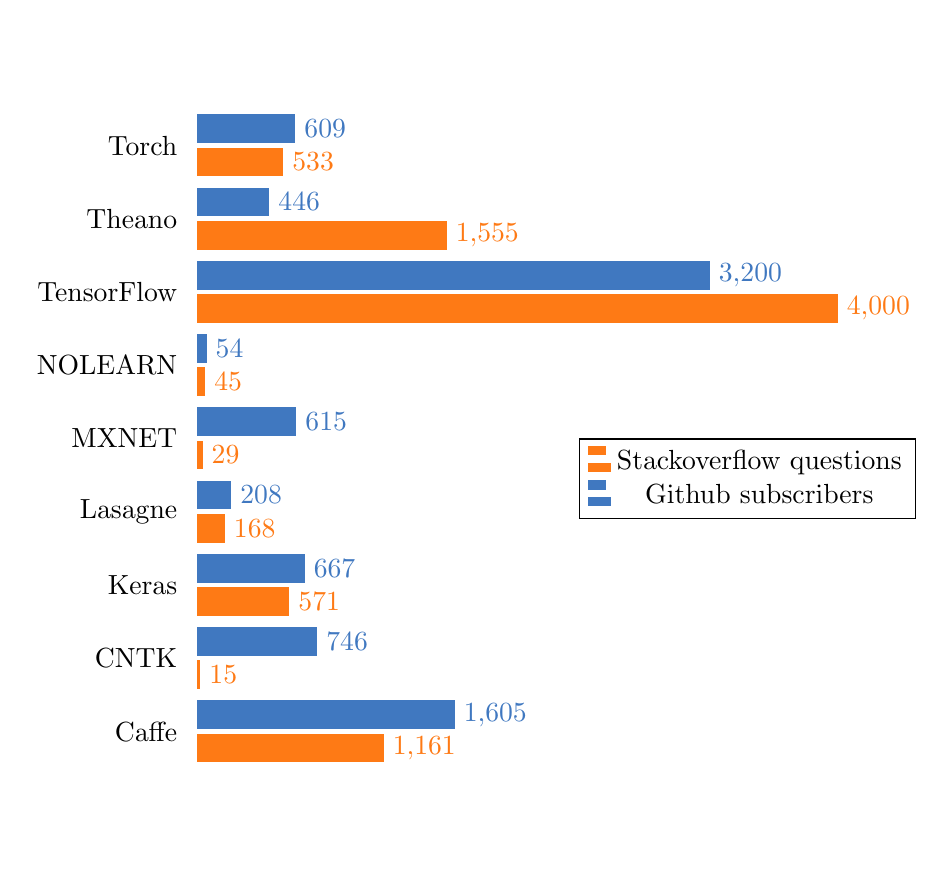
\begin{tikzpicture}
\begin{axis}[
	xbar,
	y axis line style = { opacity = 0 },
	axis x line = none,
	tickwidth = 0pt,
	enlarge y limits = 0.2,
	enlarge x limits = 0.02,
	symbolic y coords = {Caffe, CNTK, Keras, Lasagne, MXNET, NOLEARN, TensorFlow, Theano, Torch},
	ytick = data,
	nodes near coords,
	height = 12cm,
	legend style={at={(1.1, 0.5)},anchor=north east}
    ]

% stackoverflow
\addplot[color=clstackoverflow, fill=clstackoverflow] coordinates{(1161,Caffe) (15,CNTK) (571,Keras) (168,Lasagne) (29,MXNET) (45,NOLEARN) (4000,TensorFlow) (1555,Theano) (533,Torch)};

% github
\addplot[color=clgithub, fill=clgithub] coordinates{(1605,Caffe) (746,CNTK) (667,Keras) (208,Lasagne) (615,MXNET) (54,NOLEARN) (3200,TensorFlow) (446,Theano) (609,Torch)};

\legend{Stackoverflow questions, Github  subscribers}

\end{axis}
\end{tikzpicture}

\caption{\label{fig:framework_popularity}Popularity of deep learning frameworks as of October 2016.}
\end{figure}

Licensing is another important issue. All deep learning libraries presented here are distributed under one of the following open-source licenses~\cite{Rosen:2004:OSL:1014911}: MIT, Apache and BSD. The only exception is CNTK which also has a permissive license but has not adopted any of the more conventional licenses.

One should also mention deep learning libraries that are built on top of other libraries to make more a user friendly API. Lasagne and Keras~\cite{chollet2015keras} are such examples. Lasagne is built on top of Theano, Keras is built on top of both Theano and TensorFlow. It is easy to switch backend from Theano to TensorFlow and vice versa in Keras which makes it a very powerful tool. Keras API is lightweight and simple which makes it a great prototyping tool. A clear drawback of such \blockquote{on-top} libraries is a lag between introduction of new functionality in primary libraries and in on-top libraries. Furthermore, additional layers of abstraction might reduce performance. 

It is worth to mention that the list of deep learning software tools from Table~\ref{tbl:comparison_of_dl_lib} is just a small fraction of all available tools. I decided to include only those tools that are well established in terms of documentation, community support and developer's reputation. This absolutely does not mean that other tools are of poor quality, but their learning curve might be steeper compared to the well established tools.

When it comes to programming language APIs, Python is a primary choice of the majority of deep learning tools. Nearly all tools mentioned in this report have well documented extensive Python APIs. Linux is the preferred operating system for deep learning environments. As of October 2016 not all deep learning tools provide versions for Windows, while Linux is supported by all of them. It might be an issue for Vironova as its software is developed for Windows operating system. There is a number of machine learning frameworks available for Microsoft .NET framework and one of the most promising is Accord.NET~\cite{accordnet}. However at the time of writing it does not provide CNN functionality and its community support and development resources can not be compared to the leading deep learning tools. 

All experiments presented in this project have been performed using TensorFlow and Keras software tools on a machine with Linux operating system. Currently TensorFlow has no version for Windows however Keras allows to switch between TensorFlow and Theano backend, so all experiments can be replicated on a Windows machine after switching to Theano backend.

\begin{landscape}
\begin{center}
\captionof{table}{Comparison of characteristics of deep learning frameworks}
\label{tbl:comparison_of_dl_lib}
\begin{tabular}{lccccccccl}
\hline 
 & \multicolumn{2}{c}{\cellcolor{linux}Linux} & \multicolumn{2}{c}{\cellcolor{windows}Windows} & \multicolumn{2}{c}{\cellcolor{macos}Mac OS} & \multicolumn{2}{c}{Language bindings} &  \\ 
 & \cellcolor{linux}CPU & \cellcolor{linux}GPU & \cellcolor{windows}CPU & \cellcolor{windows}GPU & \cellcolor{macos}CPU & \cellcolor{macos}GPU & Python & C++ & License\\ 
\hline 
Caffe & \ymark & \ymark & \ymark & \ymark & \ymark & \ymark & \ymark & \nmark & BSD 2\\ 
CNTK & \ymark & \ymark & \ymark & \ymark & \nmark & \nmark & \ymark & \ymark & Permissive \\ 
Keras & \ymark & \ymark & \ymark & \ymark & \ymark & \ymark & \ymark & \nmark & MIT \\ 
Lasagne & \ymark & \ymark & \ymark & \ymark & \ymark & \ymark & \ymark & \nmark & MIT \\ 
MXNET & \ymark & \ymark & \ymark & \ymark & \ymark & \ymark & \ymark & \ymark & Apache 2.0 \\ 
NOLEARN & \ymark & \ymark & \ymark & \ymark & \ymark & \ymark & \ymark & \nmark & MIT \\ 
TensorFlow & \ymark & \ymark & \nmark & \nmark & \ymark & \nmark & \ymark & \ymark & Apache 2.0 \\ 
Theano & \ymark & \ymark & \ymark & \ymark & \ymark & \ymark & \ymark & \nmark & BSD 3\\ 
Torch & \ymark & \ymark & \ymark & \ymark & \ymark & \ymark & \nmark & \ymark & BSD 3\\ 
\end{tabular} 
\end{center}


\end{landscape}

\section{Network Architectures}

Five architectures are tested in this project. I start with the simplest configuration possible --- one convolutional layer followed by two fully connected layers and gradually add additional convolutional layers. Let us call the networks LipNet-\textit{x}, see Figure~\ref{fig:lipnet_arch}, where \textit{x} stands for the number of convolutional layers. 

\begin{itemize}
\item \textbf{LipNet--1} is the simplest possible configuration and a starting point for the experiments. It consists of one convolutional block with max pooling and dropout followed by two fully connected layers.

\item \textbf{LipNet--2} is an extension of LipNet--1 with one additional convolutional block. 

\item \textbf{LipNet--4} is mainly inspired by VGG--11 architecture. Two convolutional blocks with max-pooling and dropout are followed by a fully connected layer. All convolutional layers have the ReLU activation function, the \textit{same} padding mode, $3 \times 3$ filter size, 32 channels and stride equal to 1. The input size is fixed to $28 \times 28$ pixels.

\item \textbf{LipNet--4c} is inspired by ideas of fully convolutional networks and replaces max-pooling with convolution with a stride as in~\cite{DBLP:journals/corr/SpringenbergDBR14}. So max-pooling layers are replaced with convolutional layers with $2 \times 2$ stride, flatten operation is replaced with $1 \times 1$ convolution with $3$ channels. Input size is fixed to $28 \times 28$ pixels.

\item \textbf{LipNet-6} is a modification of LipNet--4 with an additional convolutional block. Additional convolution with stride requires bigger input size so images are resized to $32 \times 32$ pixels. 
\end{itemize}

Classes are one-hot encoded~\cite{harris2013digital} as demonstrated in Table~\ref{table:class_encoding}.

\begin{center}
\captionof{table}{Class encodings}
\label{table:class_encoding}
\begin{tabular}{|lc|}
\toprule 
Class & Encoding \\ 
\midrule 
Multilamellar & \texttt{100} \\ 
Unilamellar & \texttt{010} \\ 
Uncertain & \texttt{001} \\ 
\midrule 
Empty & \texttt{100} \\ 
Full & \texttt{010} \\ 
Uncertain & \texttt{001} \\ 
\bottomrule 
\end{tabular} 
\end{center}

Thus output, the layer is always represented by three nodes and each of them yields a value between 0 and 1 that is interpreted as a probability of belonging to a corresponding class. Softmax~\cite{Bishop:2006:PRM:1162264} activation function guarantees that all node values are in the range $[0, 1]$ and sum up to 1. 

\begin{figure}[H]
\centering
\includegraphics[width=\textwidth]{lipnet_architecture.png} 
\caption{Network configurations that have been tested in this project. All networks assume \textit{same} padding mode, unit stride and ReLU activations.}
\label{fig:lipnet_arch}
\end{figure}

Figure~\ref{fig:lipnet4_filters} shows an example of visualized convolutional filters of the trained LipNet--4 model. Filters are visualized with a seismic color map in order to clearly see negative and positive values: blue color corresponds to values less than zero; red --- greater than zero and finally white corresponds to zero values. 

\begin{figure}[H]
\centering
\begin{tabular}{cc}
	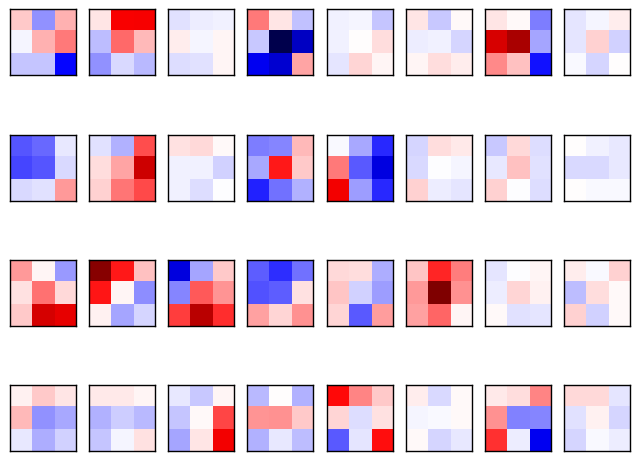
\includegraphics[width=0.45\textwidth]{models/cnn_deep/weights/convolution2d_1-0.png} & 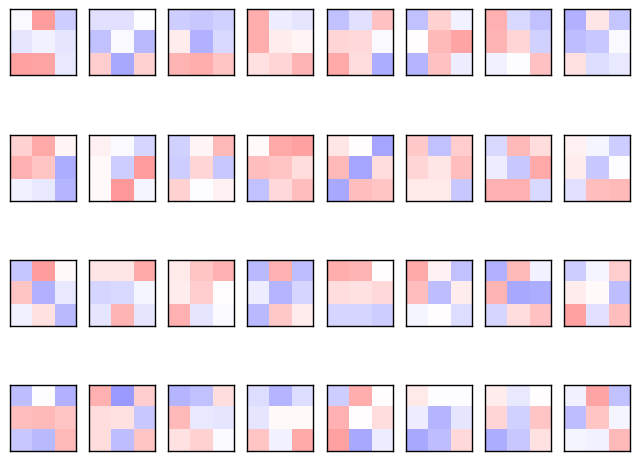
\includegraphics[width=0.45\textwidth]{models/cnn_deep/weights/convolution2d_2-23.png} \\
	\rom{1} & \rom{2}, channel 24 \\[6pt]
	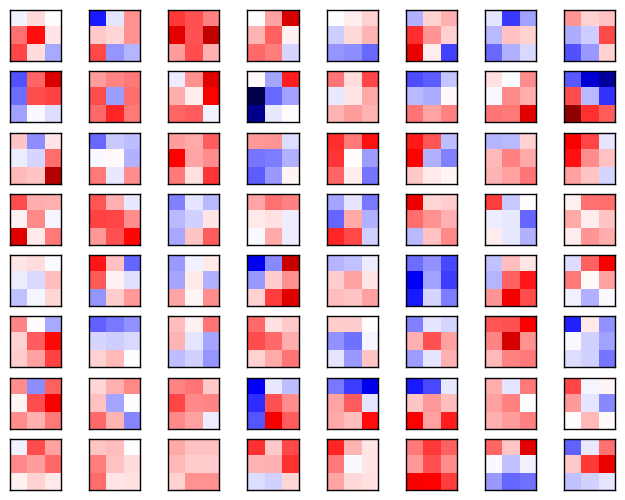
\includegraphics[width=0.45\textwidth]{models/cnn_deep/weights/convolution2d_3-3.png} & 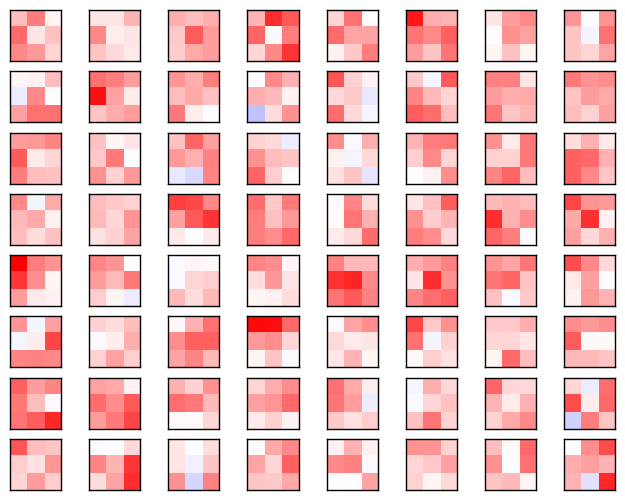
\includegraphics[width=0.45\textwidth]{models/cnn_deep/weights/convolution2d_4-58.png} \\
	\rom{3}, channel 4 & \rom{4}, channel 59 \\[6pt]
\end{tabular}
\caption{Visualization of convolution kernels}
\label{fig:lipnet4_filters}
\end{figure}

%\newpage

Figure~\ref{fig:lipnet4_conv_output} shows example output of different convolutional layers of LipNet--4 model.

\begin{figure}[H]
\centering
\begin{tabular}{cc}
	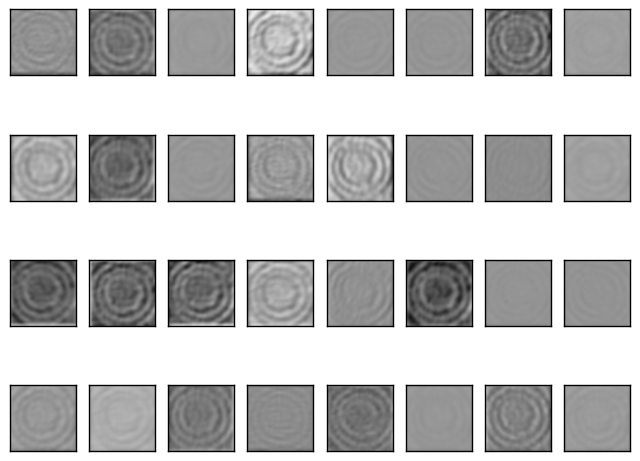
\includegraphics[width=0.45\textwidth]{models/cnn_deep/output/convolution2d_1.png} & 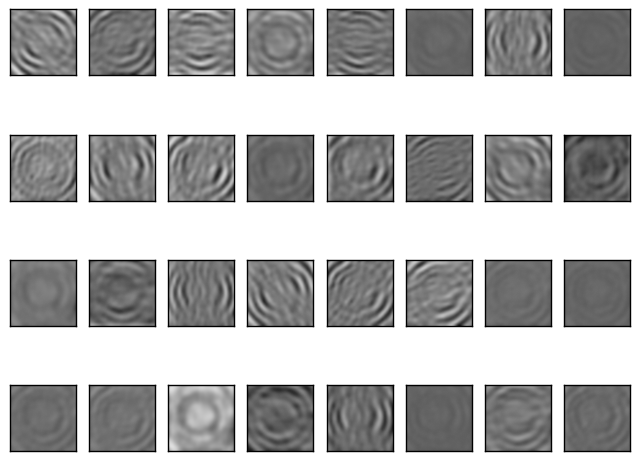
\includegraphics[width=0.45\textwidth]{models/cnn_deep/output/convolution2d_2.png} \\
	\rom{1} & \rom{2} \\[6pt]
		\includegraphics[width=0.45\textwidth]{models/cnn_deep/output/convolution2d_3.png} & \includegraphics[width=0.45\textwidth]{models/cnn_deep/output/convolution2d_4.png} \\
	\rom{3} & \rom{4} \\[6pt]

\end{tabular}
\caption{Visualization of the output from the convolutional layers.}
\label{fig:lipnet4_conv_output}
\end{figure}

\newpage
\section{Results}

\subsection{Experiment set-up}

LipNet networks were trained using Keras deep learning library with GPU based Tensorflow backend on a Linux machine. Keras allows to easily switch backend between Tensorflow and Theano so it is possible to run the same code in Windows environment as well. It takes between 60 and 130 seconds per epoch to train LipNet models on a machine with a GeForce 940M video card. GPU utilization statistics, see Figure~\ref{fig:nvidia_smi}, is invoked using the \texttt{nvidia-smi} command on Linux.

\begin{figure}[H]
\centering
\includegraphics[width=\textwidth]{nvidia_smi.png} 
\caption{GPU utilization statistics.}
\label{fig:nvidia_smi}
\end{figure}

All models are evaluated using a 5-fold cross-validation~\cite{Kohavi:1995:SCB:1643031.1643047} technique. The data is split into 5 folds using stratified sampling which means that class proportions are preserved. One fold is used as the test set while the four others as training set and the experiment is repeated five times, each time with a new fold as the test set.

Training sets are balanced using oversampling while test sets are left unbalanced. During training, the training data is augmented as described in~\ref{sec:data_augmentation}. Data augmentation transformations are applied randomly to each training example, so the probability to see  the same training example twice is quite low. 

Input samples are shuffled at the beginning of each epoch. Training data is fed in batches and model parameters are updated after each batch. Batch size is fixed to the default value of 32 images. If a validation set is used, then one can see that at the end of some epochs the validation error is less than the test error. This happens because the model parameters are updated after each batch, so validation which is done at the end of each epoch is performed after training on the whole training set, while test error is an average error of all batches within an epoch.

 

\subsection{Evaluation of data augmentation techniques}

Evaluation of the data augmentation techniques is performed in the following way. All data is divided in five folds with preserved class proportion. In turn, each of them serves as a test set while the other four constitute a training set. All training sets are balanced using oversampling, test sets are not balanced.The  Model architecture is the LipNet-4. Images contain only liposome objects, i.e. no liposome surrounding, and masks are not applied.

The first experiment is performed without any data augmentation, this corresponds to the first $x$ axis tick which is \textit{None}. Then, experiments are repeated adding augmentation techniques successively. For example \textit{Flip} tick means that this experiment was performed using \textit{Rotation}, \textit{Shift} and \textit{Flip} techniques.

The $y$ axis in Figure~\ref{fig:augmentation_evaluation} represents five-fold average normalized true positive rate for each respective class. 

\begin{figure}[H]
\centering

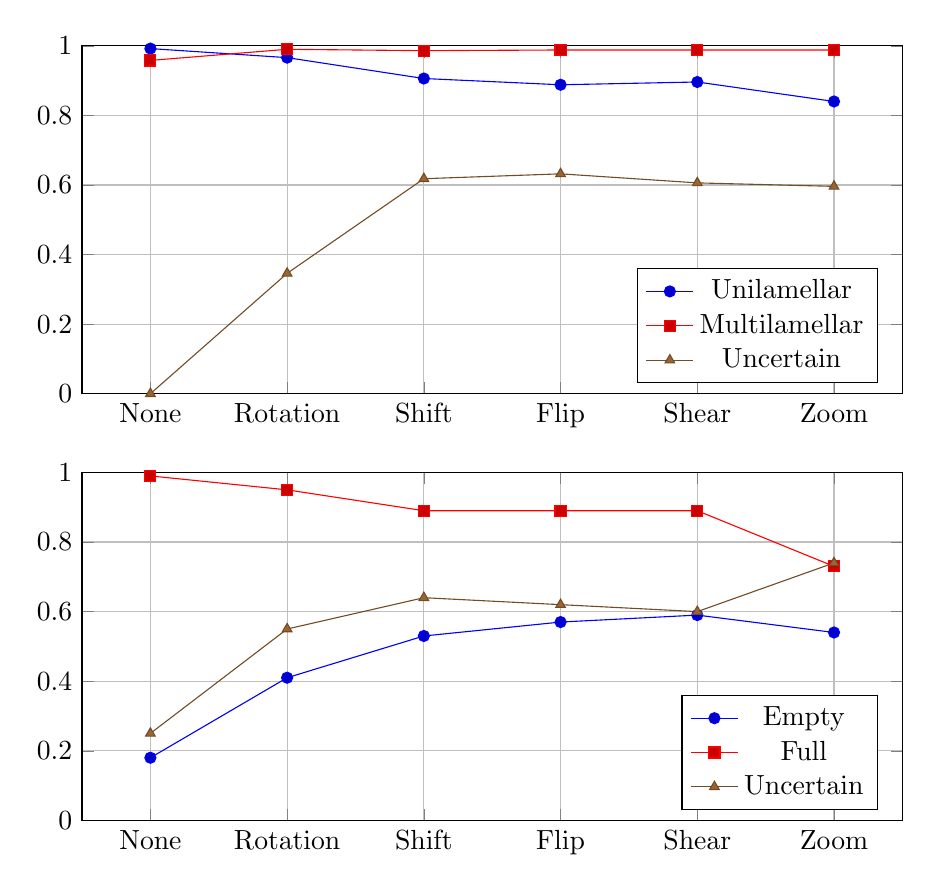
\begin{tikzpicture}
\begin{groupplot}[
	group style = {group size = 1 by 2, vertical sep=1cm,},
	width = 12cm,
	height = 6cm,
	grid=major,
    ymin=0.0,
    ymax=1.0,
    %ylabel=Average normalized true positive rate, 
    legend pos=south east,
    symbolic x coords={None, Rotation, Shift, Flip, Shear, Zoom},
    xtick=data,
    ]

% lamellarity
\nextgroupplot
\addplot+ [mark=*] coordinates{(None, 0.992) (Rotation, 0.966) (Shift, 0.906) (Flip, 0.888) (Shear, 0.896) (Zoom, 0.84)};
\addplot+ [mark=square*] coordinates{(None, 0.958) (Rotation, 0.99) (Shift, 0.986) (Flip, 0.988) (Shear, 0.988) (Zoom, 0.988)};
\addplot+ [mark=triangle*] coordinates{(None, 0.0) (Rotation, 0.346) (Shift, 0.618) (Flip, 0.632) (Shear, 0.606) (Zoom, 0.596)};

\legend{Unilamellar, Multilamellar, Uncertain}

% encapsulation
\nextgroupplot
\addplot+ [mark=*] coordinates{(None, 0.18) (Rotation, 0.41) (Shift, 0.53) (Flip, 0.57) (Shear, 0.59) (Zoom, 0.54)};
\addplot+ [mark=square*] coordinates{(None, 0.99) (Rotation, 0.95) (Shift, 0.89) (Flip, 0.89) (Shear, 0.89) (Zoom, 0.73)};
\addplot+ [mark=triangle*] coordinates{(None, 0.25) (Rotation, 0.55) (Shift, 0.64) (Flip, 0.62) (Shear, 0.6) (Zoom, 0.74)};
\legend{Empty, Full, Uncertain}

\end{groupplot}
\end{tikzpicture}

\caption{\label{fig:augmentation_evaluation}Effect of combining augmentation techniques successively on the average normalized true positive rate. Top --- Lamellarity problem, bottom --- Encapsulation.}
\end{figure}

In the \textbf{lamellarity} problem, the clear benefit of data augmentation is for the \textit{uncertain} class. The majority  class \textit{unilamellar} and the runner up \textit{multilamellar} are being classified with almost $100\%$ accuracy even without any augmentation of training data. However the \textit{uncertain} class is totally misclassified when no augmentation is performed. Rotation itself raises the true positive rate of \textit{uncertain} to nearly $40\%$ which makes sense. Considering the very small number (84) of examples in this class, it is not an unlikely scenario when the test set contains patterns that the model has not seen during training. For example the train and test set contain patterns that are similar but differently oriented. In such a case, rotation improves the result a lot which is the case in this experiment. Adding shift transformation brings further improvement to recognition of \textit{uncertain} class objects. Adding flip, shear and zoom transformations do not have any positive effect on performance. In fact, more aggressive data augmentation worsens the model's ability to generalize and the performance on \textit{unilamellar} and \textit{uncertain} classes drops a bit when all transformations are used.

The \textbf{encapsulation} data is even more unbalanced than the lamellarity data, so without any data augmentation almost all examples are classified as \textit{full}. Data augmentation makes clear improvement in performance, the true positive rates of the \textit{empty} and \textit{uncertain} classes are increasing while \textit{full} slowly decreases from approximately $1.0$ to $0.9$ as rotation and shift transformations are employed. Adding additional transformations do not improve performance and the trend is quite similar to the one observed in the lamellarity problem except the the last point. Adding zoom transformation improves the model's ability to recognize \textit{uncertain} examples while it worsens the performance on \textit{full} examples. This is an unexpected result, since it would be natural to expect general performance improvement when zoom transformation is used. Zoom encourages the model to focus more on the core of the liposome which is the most relevant part in the encapsulation problem.

In order to analyze the effect of zoom transformation in more detail an additional experiment was performed. This time the data was augmented using only zoom transformation. Results are presented in Table~\ref{table:zoom_only}. The performance is approximately equal to rotation-only augmentation. 

\begin{center}
\captionof{table}{5-fold average normalized confusion matrix, encapsulation problem, zoom only.}
\label{table:zoom_only}
\begin{tabular}{|L{2.5cm} |C{2.5cm} |C{2.5cm} |C{2.5cm}|}
\toprule
 & Empty & Full & Uncertain \\
\midrule
Empty & 0.43 & 0.13 & 0.44 \\
Full & 0.04 & 0.90 & 0.06 \\
Uncertain & 0.14 & 0.35 & 0.51 \\
\bottomrule
\end{tabular}
\end{center}

The best option would be to evaluate all possible combinations of transformations applied in all possible orders but that would require to run 325 experiments. Unfortunately due to hardware and time limitations it is not feasible to perform such a number of experiments.

\subsection{Evaluation of different CNN models}

In this section different LipNet models are evaluated and compared. The average $F_1$ score is recorded for each class.

Results for Lamellarity problem are shown in Figure~\ref{fig:cnn_models_lamellarity}. LipNet-4 is a clear leader that outperforms all other models for all classes. It is interesting to note that multilamellar liposomes are recognized by LipNet-4 with almost no error despite the fact that only $12\%$ of all particles in the data set belong to that class compared to $87\%$ of unilamellar particles. All other models demonstrated more or less similar results regarding recognition of unilamellar and multilamellar liposomes. LipNet-4 and LipNet-6 were the best to recognize particles of the uncertain class clearly outperforming the other models.

\begin{figure}[H]
\centering

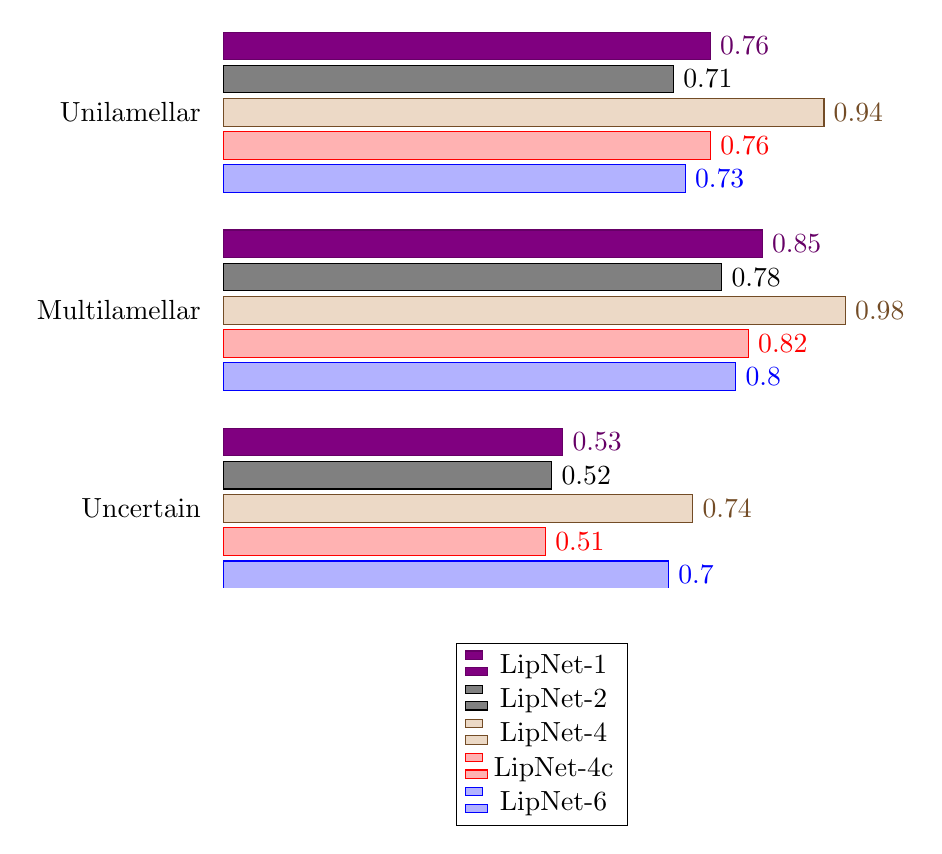
\begin{tikzpicture}
\begin{axis}[
	xbar,
	reverse legend,
	y axis line style = { opacity = 0 },
	axis x line = none,
	tickwidth = 0pt,
	enlarge y limits = 0.2,
	enlarge x limits = 0.02,
	symbolic y coords = {Uncertain, Multilamellar, Unilamellar},
	ytick = data,
	nodes near coords,
	legend style={at={(0.5, -0.1)},anchor=north},
	xmin=0,
	xmax=1,
    ]

% LipNet-6
\addplot coordinates{(0.6987,Uncertain) (0.8041,Multilamellar) (0.7250,Unilamellar)};
\addlegendentry{LipNet-6}

% LipNet-4c
\addplot coordinates{(0.5057,Uncertain) (0.8240,Multilamellar) (0.7645,Unilamellar)};
\addlegendentry{LipNet-4c}

% LipNet-4
\addplot coordinates{(0.7367,Uncertain) (0.9762,Multilamellar) (0.9425,Unilamellar)};
\addlegendentry{LipNet-4}

% LipNet-2
\addplot coordinates{(0.5156,Uncertain) (0.7823,Multilamellar) (0.7065,Unilamellar)};
\addlegendentry{LipNet-2}

% LipNet-1
\addplot coordinates{(0.5327,Uncertain) (0.8458,Multilamellar) (0.7641,Unilamellar)};
\addlegendentry{LipNet-1}

\end{axis}
\end{tikzpicture}

\caption{\label{fig:cnn_models_lamellarity}Lamellarity problem. $F_1$ scores for different CNN models.}
\end{figure}

Results for the encapsulation problem are shown in Figure~\ref{fig:cnn_models_encapsulation}. Unlike the lamellarity problem there is no clear leader, so no model outperforms the other for all classes. Simpler models like LipNet-1 and LipNet-2 are superior when it comes to the \textit{empty} class but they are marginally worse than LipNet-4 and LipNet-4c in recognizing the \textit{full} class. LipNet-4 and LipNet-4c are best at recognizing liposomes of the \textit{uncertain} class, but the LipNet-1 result is very close. The only clear pattern is that LipNet-6's ability to generalize is the worst among all tested models. It probably has to many parameters and overfits which leads to poor generalization.

\begin{figure}[H]
\centering

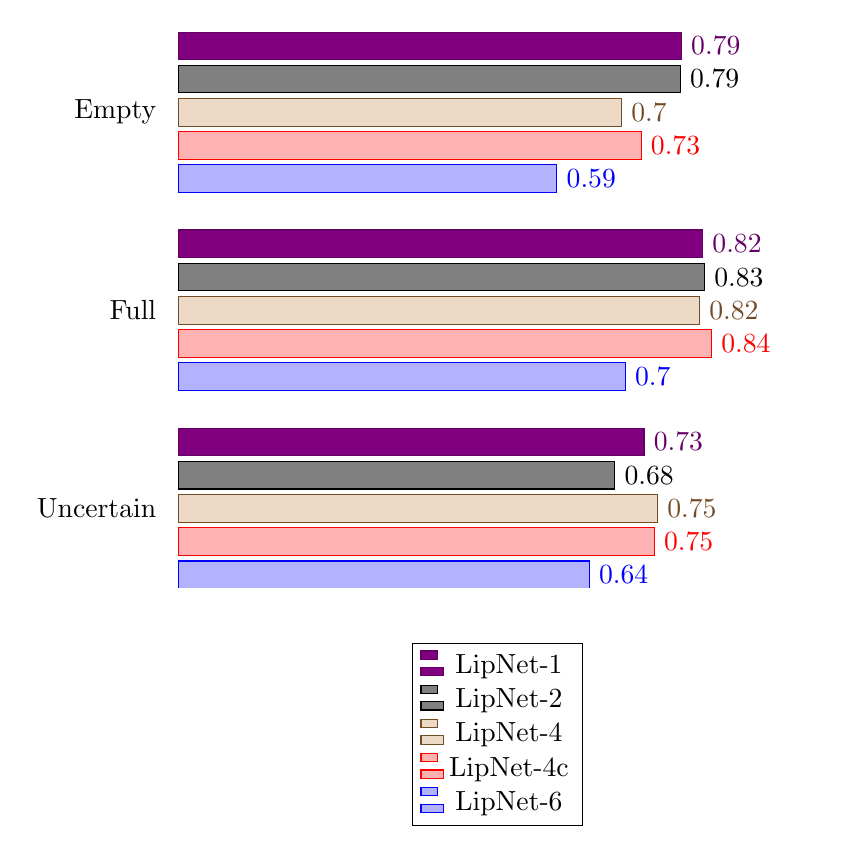
\begin{tikzpicture}
\begin{axis}[
	xbar,
	reverse legend,
	y axis line style = { opacity = 0 },
	axis x line = none,
	tickwidth = 0pt,
	enlarge y limits = 0.2,
	enlarge x limits = 0.02,
	symbolic y coords = {Uncertain, Full, Empty},
	ytick = data,
	nodes near coords,
	legend style={at={(0.5, -0.1)},anchor=north},
	xmin=0,
	xmax=1,
    ]

% LipNet-6
\addplot coordinates{(0.5935,Empty) (0.7008,Full) (0.6442,Uncertain)};
\addlegendentry{LipNet-6}

% LipNet-4c
\addplot coordinates{(0.7257,Empty) (0.8360,Full) (0.7463,Uncertain)};
\addlegendentry{LipNet-4c}

% LipNet-4
\addplot coordinates{(0.6950,Empty) (0.8172,Full) (0.7514,Uncertain)};
\addlegendentry{LipNet-4}

% LipNet-2
\addplot coordinates{(0.7870,Empty) (0.8250,Full) (0.6843,Uncertain)};
\addlegendentry{LipNet-2}

% LipNet-1
\addplot coordinates{(0.7889,Empty) (0.8222,Full) (0.7301,Uncertain)};
\addlegendentry{LipNet-1}

\end{axis}
\end{tikzpicture}

\caption{\label{fig:cnn_models_encapsulation}Encapsulation problem. $F_1$ scores for different CNN models.}
\end{figure}

%\begin{landscape}
%\begin{table}
%\caption{5-fold cross validation, LipNet--4, Lamellarity problem.} \label{t:kfold-cnn-lamellarity}
%
%\smallskip
%\begin{tabular*}{\linewidth}{@{} l @{\extracolsep{\fill}} *{12}{S[table-format=2.1]}
%                                 *{4}{S[table-format=2.1]} @{}}
%\toprule
% & \multicolumn{4}{c}{Unilamellar} & \multicolumn{4}{c}{Multilamellar} 
%         & \multicolumn{4}{c}{Uncertain}  \\
%\cmidrule(lr){2-5} \cmidrule(lr){6-9} \cmidrule(lr){10-13}  
%Fold & \mcc{TPR} & \mcc{SPC} & \mcc{PPV} & \mcc{NPV} & \mcc{TPR} & \mcc{SPC} & \mcc{PPV} & \mcc{NPV} & \mcc{TPR} & \mcc{SPC} & \mcc{PPV} & \mcc{NPV}  \\
%\midrule
%1 & 0.8634 & 0.9972 & 0.9995 & 0.5158 & 0.9797 & 0.9542 & 0.7472 & 0.9971 & 0.5294 & 0.9155 & 0.0364 & 0.9969\\
%2 & 0.9107 & 0.9917 & 0.9987 & 0.6183 & 0.9913 & 0.9683 & 0.8119 & 0.9988 & 0.4706 & 0.9464 & 0.0503 & 0.9966\\
%3 & 0.9798 & 0.9945 & 0.9992 & 0.8778 & 1.0000 & 0.9912 & 0.9399 & 1.0000 & 0.4706 & 0.9876 & 0.1860 & 0.9968\\
%4 & 0.9915 & 0.9945 & 0.9992 & 0.9447 & 0.9884 & 0.9972 & 0.9798 & 0.9984 & 0.8235 & 0.9933 & 0.4242 & 0.9989\\
%5 & 0.8956 & 0.9972 & 0.9995 & 0.5798 & 0.9707 & 0.9803 & 0.8711 & 0.9959 & 0.7500 & 0.9211 & 0.0513 & 0.9985\\
%\midrule
%Avg & 0.9282 & 0.9950 & 0.9992 & 0.7073 & 0.9860 & 0.9782 & 0.8700 & 0.9980 & 0.6088 & 0.9528 & 0.1497 & 0.9975\\ 
%\bottomrule
%\end{tabular*}
%\end{table}
%
%\begin{table}
%\caption{5-fold cross validation, LipNet--4, Encapsulation problem.} \label{t:kfold-cnn-encapsulation}
%
%\smallskip
%\begin{tabular*}{\linewidth}{@{} l @{\extracolsep{\fill}} *{12}{S[table-format=2.1]}
%                                 *{4}{S[table-format=2.1]} @{}}
%\toprule
% & \multicolumn{4}{c}{Empty} & \multicolumn{4}{c}{Full} 
%         & \multicolumn{4}{c}{Uncertain}  \\
%\cmidrule(lr){2-5} \cmidrule(lr){6-9} \cmidrule(lr){10-13}  
%Fold & \mcc{TPR} & \mcc{SPC} & \mcc{PPV} & \mcc{NPV} & \mcc{TPR} & \mcc{SPC} & \mcc{PPV} & \mcc{NPV} & \mcc{TPR} & \mcc{SPC} & \mcc{PPV} & \mcc{NPV}  \\
%\midrule
%1 & 0.3030 & 0.9917 & 0.1961 & 0.9953 & 0.8194 & 0.8358 & 0.9945 & 0.1134 & 0.7624 & 0.8239 & 0.0822 & 0.9941\\
%2 & 0.3030 & 0.9861 & 0.1266 & 0.9953 & 0.9019 & 0.7761 & 0.9932 & 0.1793 & 0.5149 & 0.9081 & 0.1038 & 0.9891\\
%3 & 0.4545 & 0.9849 & 0.1667 & 0.9963 & 0.8992 & 0.8955 & 0.9968 & 0.1970 & 0.7030 & 0.9083 & 0.1368 & 0.9933\\
%4 & 0.6061 & 0.9895 & 0.2778 & 0.9974 & 0.9427 & 0.7836 & 0.9937 & 0.2742 & 0.6139 & 0.9490 & 0.1994 & 0.9917\\
%5 & 0.8276 & 0.9861 & 0.2581 & 0.9990 & 0.9258 & 0.9291 & 0.9980 & 0.2469 & 0.5510 & 0.9322 & 0.1403 & 0.9904\\
%\midrule
%Avg & 0.4989 & 0.9876 & 0.2050 & 0.9967 & 0.8978 & 0.8440 & 0.9952 & 0.2021 & 0.6290 & 0.9043 & 0.1325 & 0.9917\\ 
%\bottomrule
%\end{tabular*}
%\end{table}
%
%\end{landscape}

\subsection{SVM}
SVM is currently used by Vironova for automatic classification and it is included in this project for benchmarking purposes. No additional experiments were performed, just those that were necessary to replicate Vironovas result. 
The following features are used to train the SVM models.
\begin{itemize}
\item Area
\item Circularity
\item Image moments $\mu_{20}$, $\mu_{02}$, $\mu_{30}$, $\mu_{03}$
\item Edge density profile
\item Histogram
\item Internal segmentation variance
\end{itemize}

The input data is divided into the training and test sets in the same way as for the CNN's experiments. However training sets are not balanced this time, instead class weights are adjusted inversely proportional to the class frequencies in the input data.

Tables~\ref{table:svm_cf_avg_encapsulation} and~\ref{table:svm_cf_avg_lamellarity} present average normalized confusion matrices for the encapsulation and lamellarity problems, respectively. Data sets are so unbalanced that total accuracy coincides with the true positive rate for the majority classes, which are \textit{empty} and \textit{unilamellar}, respectively. 

\begin{center}
\captionof{table}{5-fold average normalized confusion matrix for the encapsulation problem using the SVM classifier.}
\label{table:svm_cf_avg_encapsulation}
\begin{tabular}{|L{2.5cm} |C{2.5cm} |C{2.5cm} |C{2.5cm}|}
\toprule
 & Empty & Full & Uncertain \\
\midrule
Empty & 0.89 & 0.01 & 0.10 \\
Full & 0.04 & 0.87 & 0.09 \\
Uncertain & 0.18 & 0.10 & 0.72 \\
\bottomrule
\end{tabular}
\end{center}

\begin{center}
\captionof{table}{5-fold average normalized confusion matrix for the lamellarity problem using the SVM classifier.}
\label{table:svm_cf_avg_lamellarity}
\begin{tabular}{|L{2.5cm} |C{2.5cm} |C{2.5cm} |C{2.5cm}|}
\toprule
 & Unilamellar & Multilamellar & Uncertain \\
\midrule
Unilamellar & 0.94 & 0.04 & 0.02 \\
Multilamellar & 0.00 & 0.98 & 0.02 \\
Uncertain & 0.03 & 0.11 & 0.86 \\
\bottomrule
\end{tabular}
\end{center}

%\begin{landscape}
%
%\begin{table}
%\caption{5-fold cross validation, SVM, Lamellarity problem.} \label{t:kfold-svm-lamellarity}
%
%\smallskip
%\begin{tabular*}{\linewidth}{@{} l @{\extracolsep{\fill}} *{12}{S[table-format=2.1]}
%                                 *{4}{S[table-format=2.1]} @{}}
%\toprule
% & \multicolumn{4}{c}{Unilamellar} & \multicolumn{4}{c}{Multilamellar} 
%         & \multicolumn{4}{c}{Uncertain}  \\
%\cmidrule(lr){2-5} \cmidrule(lr){6-9} \cmidrule(lr){10-13}  
%Fold & \mcc{TPR} & \mcc{SPC} & \mcc{PPV} & \mcc{NPV} & \mcc{TPR} & \mcc{SPC} & \mcc{PPV} & \mcc{NPV} & \mcc{TPR} & \mcc{SPC} & \mcc{PPV} & \mcc{NPV}  \\
%\midrule
%1 & 0.8659 & 0.9812 & 0.9969 & 0.5157 & 0.9527 & 0.9736 & 0.8326 & 0.9933 & 0.9851 & 0.9021 & 0.0565 & 0.9999 \\
%2 & 0.8578 & 0.9826 & 0.9971 & 0.5014 & 0.9432 & 0.9719 & 0.8222 & 0.9920 & 0.9701 & 0.8951 & 0.0521 & 0.9998 \\
%3 & 0.8404 & 0.9806 & 0.9966 & 0.4721 & 0.9432 & 0.9671 & 0.7979 & 0.9920 & 0.9701 & 0.8844 & 0.0475 & 0.9998  \\
%4 & 0.8742 & 0.9757 & 0.9960 & 0.5302 & 0.9315 & 0.9721 & 0.8215 & 0.9904 & 0.9851 & 0.9088 & 0.0604 & 0.9999\\
%5 & 0.8651 & 0.9806 & 0.9967 & 0.5147 & 0.9477 & 0.9695 & 0.8109 & 0.9926 & 0.9706 & 0.9045 & 0.0577 & 0.9998\\
%\midrule
%Avg & 0.8607 & 0.9801 & 0.9967 & 0.5068 & 0.9436 & 0.9708 & 0.8170 & 0.9921 & 0.9762 & 0.8990 & 0.0548 & 0.9998\\ 
%\bottomrule
%\end{tabular*}
%\end{table}
%
%\begin{table}
%\caption{5-fold cross validation, SVM, Encapsulation problem.} \label{t:kfold-svm-encapsulation}
%
%\smallskip
%\begin{tabular*}{\linewidth}{@{} l @{\extracolsep{\fill}} *{12}{S[table-format=2.1]}
%                                 *{4}{S[table-format=2.1]} @{}}
%\toprule
% & \multicolumn{4}{c}{Empty} & \multicolumn{4}{c}{Full} 
%         & \multicolumn{4}{c}{Uncertain}  \\
%\cmidrule(lr){2-5} \cmidrule(lr){6-9} \cmidrule(lr){10-13}  
%Fold & \mcc{TPR} & \mcc{SPC} & \mcc{PPV} & \mcc{NPV} & \mcc{TPR} & \mcc{SPC} & \mcc{PPV} & \mcc{NPV} & \mcc{TPR} & \mcc{SPC} & \mcc{PPV} & \mcc{NPV}  \\
%\midrule
%1 & 0.8750 & 0.9594 & 0.1223 & 0.9992 & 0.8703 & 0.9357 & 0.9980 & 0.1644 & 0.7082 & 0.9073 & 0.1356 & 0.9934\\
%2 & 0.8984 & 0.9477 & 0.1000 & 0.9993 & 0.8625 & 0.9376 & 0.9980 & 0.1567 & 0.7681 & 0.9126 & 0.1529 & 0.9948\\
%3 & 0.8828 & 0.9576 & 0.1186 & 0.9992 & 0.8582 & 0.9149 & 0.9973 & 0.1496 & 0.7207 & 0.8979 & 0.1266 & 0.9937\\
%4 & 0.8516 & 0.9487 & 0.0969 & 0.9990 & 0.8676 & 0.9244 & 0.9976 & 0.1599 & 0.7980 & 0.9174 & 0.1655 & 0.9955\\
%5 & 0.9318 & 0.9570 & 0.1263 & 0.9995 & 0.8666 & 0.9067 & 0.9970 & 0.1580 & 0.6337 & 0.9056 & 0.1218 & 0.9917\\
%\midrule
%Avg & 0.8879 & 0.9541 & 0.1128 & 0.9992 & 0.8650 & 0.9239 & 0.9976 & 0.1577 & 0.7257 & 0.9082 & 0.1405 & 0.9938\\ 
%\bottomrule
%\end{tabular*}
%\end{table}
%
%\end{landscape}

%\newpage

\subsection{Impact of surrounding and masking on the input images}

Recall that each image contains a liposome object and its surrounding which goes 50 pixels in each direction. Corresponding particle masks are also available. It is hence a matter of design whether to include surrounding or not  as well as if masks are to be applied. The following three alternatives have been tested:
\begin{itemize}
\item Input images with surrounding. All images include information about particles surrounding.

\item Cropped images. All images are cropped to a minimum size allowed while still containing the liposome object.

\item Cropped and masked. All images are cropped and the corresponding masks are applied. This means that each image contains information only about a particular particle and nothing else.
\end{itemize}

The comparison is performed in terms of $F_1$ score (averaged across 5 folds) for the LipNet-4 network trained on images in the modes described above.

Results of the experiments show that including surrounding to the input images leads to worse performance in both problems for all classes. The best performance is achieved when the input images are cropped and masked. A detailed comparison is shown in Figures~\ref{fig:input_img_comparison_encapsulation} and~\ref{fig:input_img_comparison_lamellarity}.

\begin{figure}[H]
\centering

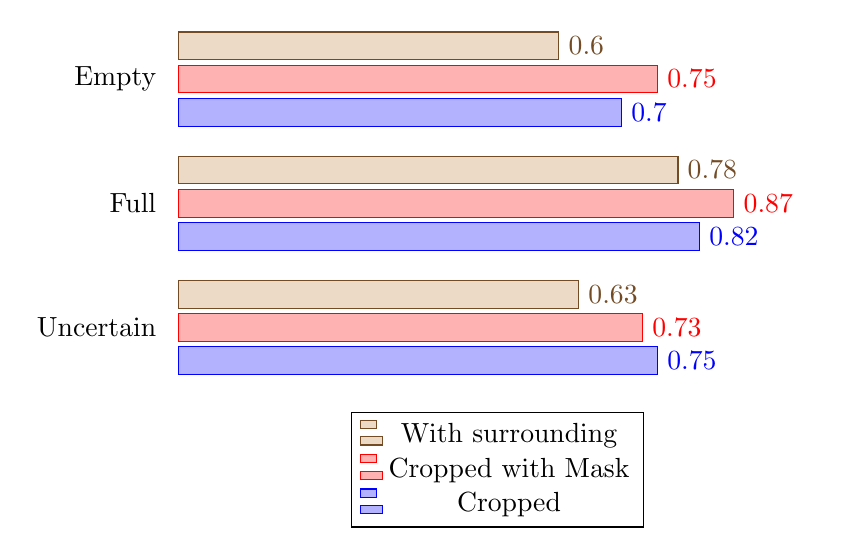
\begin{tikzpicture}
\begin{axis}[
	xbar,
	reverse legend,
	y axis line style = { opacity = 0 },
	axis x line = none,
	tickwidth = 0pt,
	enlarge y limits = 0.2,
	enlarge x limits = 0.02,
	symbolic y coords = {Uncertain, Full, Empty},
	ytick = data,
	nodes near coords,
	height = 6cm,
	legend style={at={(0.5, -0.1)},anchor=north},
	xmin=0,
	xmax=1,
    ]

% Cropped
\addplot coordinates{(0.6950,Empty) (0.8172,Full) (0.7514,Uncertain)};
\addlegendentry{Cropped}

% Cropped with mask
\addplot coordinates{(0.7515,Empty) (0.8712,Full) (0.7279,Uncertain)};
\addlegendentry{Cropped with Mask}

% With surrounding
\addplot coordinates{(0.5966,Empty) (0.7834,Full) (0.6276,Uncertain)};
\addlegendentry{With surrounding}

\end{axis}
\end{tikzpicture}

\caption{\label{fig:input_img_comparison_encapsulation}Comparison of the $F_1$ score of the LipNet-4 network with different input image modes: with surrounding, cropped, cropped and masked, for the encapsulation problem}
\end{figure}

\begin{figure}[H]
\centering

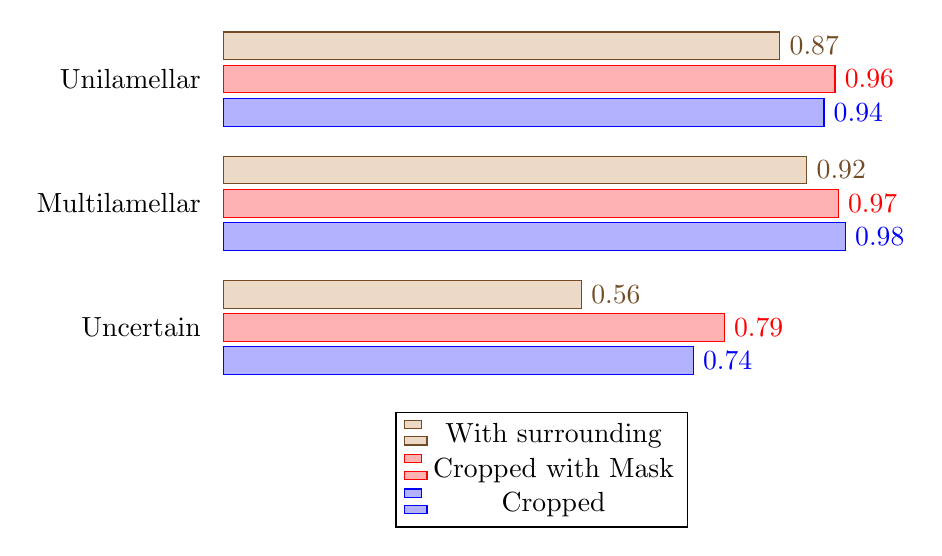
\begin{tikzpicture}
\begin{axis}[
	xbar,
	reverse legend,
	y axis line style = { opacity = 0 },
	axis x line = none,
	tickwidth = 0pt,
	enlarge y limits = 0.2,
	enlarge x limits = 0.02,
	symbolic y coords = {Uncertain, Multilamellar, Unilamellar},
	ytick = data,
	nodes near coords,
	height = 6cm,
	legend style={at={(0.5, -0.1)},anchor=north},
	xmin=0,
	xmax=1,
    ]

% Cropped
\addplot coordinates{(0.9425,Unilamellar) (0.9762,Multilamellar) (0.7376,Uncertain)};
\addlegendentry{Cropped}

% Cropped with mask
\addplot coordinates{(0.9599,Unilamellar) (0.9650,Multilamellar) (0.7862,Uncertain)};
\addlegendentry{Cropped with Mask}

% With surrounding
\addplot coordinates{(0.8734,Unilamellar) (0.9158,Multilamellar) (0.5622,Uncertain)};
\addlegendentry{With surrounding}

\end{axis}
\end{tikzpicture}

\caption{\label{fig:input_img_comparison_lamellarity}Comparison of the $F_1$ score of the LipNet-4 network with different input image modes: with surrounding, cropped, cropped and masked, for the lamellarity problem.}
\end{figure}


\newpage
\section{Benchmarking}

In this section selected CNN models are benchmarked against SVM. For each problem the CNN model that performed the best in the previous experiments has been selected for comparison to SVM. For the lamellarity problem, the LipNet-4 model has been selected, for the encapsulation problem --- LipNet-2. In both cases data sets are balanced using oversampling, the input images are cropped, masked and augmented. All performance metrics are presented in Figure~\ref{fig:svm_vs_cnn}. 

Unilamellar and multilamellar liposomes are recognized by both LipNet-4 and SVM with reasonably good results. Convolutional neural network slightly outperforms SVM in this case. In particular CNN is better in predicting that a particle is not unilamellar. The CNN's negative predicted value is $0.7$ against $0.5$ for SVM. On the other hand, results are opposite when it comes to the \textit{uncertain} class of the lamellarity problem. Here SVM clearly outperforms CNN in terms of sensitivity: SVM identifies nearly all particles of the \textit{uncertain} class while CNN does so only in $70\%$ of cases. However both methods yield many false positive predictions of the \textit{uncertain} class which results in poor precision. The CNN has almost twice the precision compared to SVM but it is still very poor being slightly above $10\%$. Mainly unilamellar liposomes are confused with uncertain ones by both CNN and SVM. Even if a small fraction of unilamellar liposomes are falsely identified as \textit{uncertain}, it is enough to bring down precision because the data sets are heavily unbalanced. The unnormalised confusion matrix averaged across 5 folds is presented in Table~\ref{table:cnn_lamellarity_cf_not_normalized}. 

\begin{figure}[H]
\centering
\captionof{table}{5-fold average unnormalised confusion matrix, Lamellarity problem, LipNet-4.}
\label{table:cnn_lamellarity_cf_not_normalized}
\begin{tabular}{|L{2.5cm} |C{2.5cm} |C{2.5cm} |C{2.5cm}|}
\toprule
 & Unilamellar & Multilamellar & Uncertain \\
\midrule
Unilamellar & 2325 & 15 & 124 \\
Multilamellar & 4 & 323 & 16 \\
Uncertain & 2 & 3 & 11 \\
\bottomrule
\end{tabular}
\end{figure}


Particles from the encapsulation problem are generally better classified by the SVM. In this case, SVM outperforms CNN for all three classes however the difference is not very big. The LipNet-2 still demonstrates a reasonable level of performance. Positive predicted values of the \textit{empty} and the \textit{uncertain} classes demonstrate the same pattern as the \textit{uncertain} class from the lamellarity problem. Approximately $10\%$ of the positive \textit{empty} predictions and $15\%$ of the positive \textit{uncertain} predictions are correct because some \textit{full} liposomes are falsely classified as either \textit{empty} or \textit{uncertain}. Once again, even if a small fraction of \textit{full} liposomes are misclassified this reduces precision of the minority classes drastically. Another notable result is the low negative predicted value of the \textit{full} class. It means that classifiers yield more false negative predictions than true negative. On the other hand the positive predicted value of both the CNN and the SVM for the \textit{full} class is almost 1 which means that there are hardly any \textit{empty} or \textit{uncertain} particles that are falsely classified as full. In other words it means that if a classifier says that a particle is \textit{full} then it is most likely \textit{full}. However, when it says the opposite it is most likely to be false. In this way the classifier is very careful in predicting a particle being \textit{full}. It would rather yield a false negative \textit{full} prediction than a false positive. It may be both good and bad depending on the domain. Discussion of risks and potential side effects of under- and overestimating the rate of liposomal encapsulation are beyond the scope of this project. 

The unnormalised confusion matrix averaged across 5 folds  is presented in Table~\ref{table:cnn_encapsulation_cf_not_normalized}.     

\begin{figure}[H]
\centering
\captionof{table}{5-fold average unnormalised confusion matrix, Encapsulation problem, LipNet-4.}
\label{table:cnn_encapsulation_cf_not_normalized}
\begin{tabular}{|L{2.5cm} |C{2.5cm} |C{2.5cm} |C{2.5cm}|}
\toprule
 & Empty & Full & Uncertain \\
\midrule
Empty & 24 & 1 & 7 \\
Full & 272 & 3929 & 660 \\
Uncertain & 30 & 9 & 61 \\
\bottomrule
\end{tabular}
\end{figure}


\begin{landscape}

\begin{figure}
\centering

% Empty
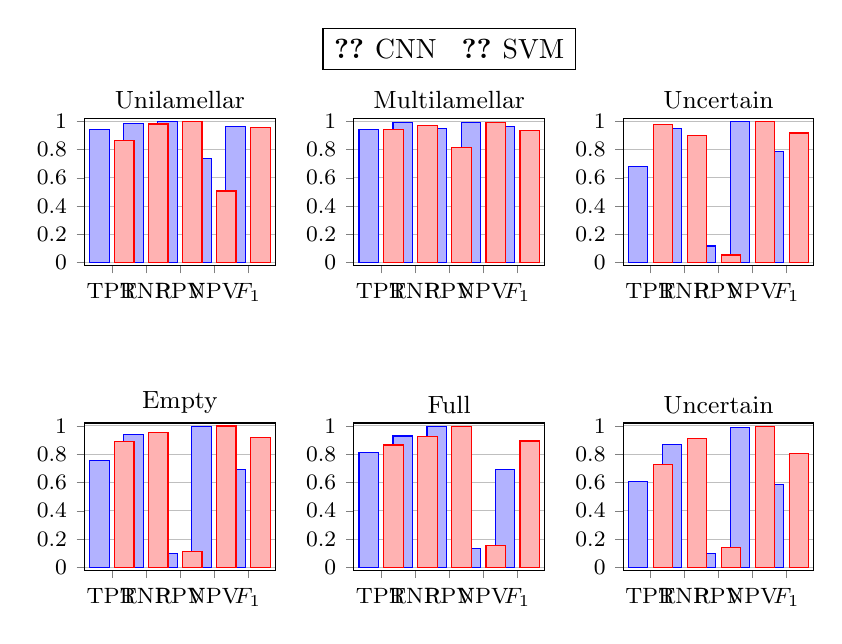
\begin{tikzpicture}
\begin{groupplot}[
	group style={
		group name=group_encapsulation,
		group size=3 by 2,
		ylabels at=edge left,
		vertical sep=2cm,
	},
	footnotesize,
	width= \linewidth * 0.33,
	%height=5cm,
	tickpos=left,
	ytick align=outside,
	xtick align=outside,
	enlarge x limits = 0.2,
	enlarge y limits = 0.02,
	xtick=data,
	enlarge x limits = 0.2,
	enlarge y limits = 0.02,
	ymin=0,
	ymax=1,
	legend style={at={(0.5,-0.1)},
	anchor=north,legend columns=-1},
	ybar,
	symbolic x coords={TPR, TNR, PPV, NPV, $F_1$},
	grid=major,
	xmajorgrids=false,
	/pgf/bar width=7pt,
]
%
% Lamlellarity
%
\nextgroupplot[title={Unilamellar}]
% lipnet-4 with mask
\addplot coordinates{(TPR, 0.9403) (TNR, 0.9817) (PPV, 0.9972) (NPV, 0.7365) ($F_1$, 0.9599)};\label{legend:cnn}

% SVM
\addplot coordinates{(TPR, 0.8607) (TNR, 0.9801) (PPV, 0.9967) (NPV, 0.5068) ($F_1$, 0.9570)};\label{legend:svm}



\nextgroupplot[title={Multilamellar}]
% lipnet-4
\addplot coordinates{(TPR, 0.9400) (TNR, 0.9921) (PPV, 0.9461) (NPV, 0.9918) ($F_1$, 0.9650)};
% svm
\addplot coordinates{(TPR, 0.9436) (TNR, 0.9708) (PPV, 0.8170) (NPV, 0.9921) ($F_1$, 0.9360)};

\nextgroupplot[title={Uncertain}]
% lipnet-4
\addplot coordinates{(TPR, 0.6801) (TNR, 0.9477) (PPV, 0.1182) (NPV, 0.9980) ($F_1$, 0.7862)};
% svm
\addplot coordinates{(TPR, 0.9762) (TNR, 0.8990) (PPV, 0.0548) (NPV, 0.9998) ($F_1$, 0.9165)};

%
% Encapsulation
%
\nextgroupplot[title={Empty}]
% lipnet-1
\addplot coordinates{(TPR, 0.7576) (TNR, 0.9384) (PPV, 0.0978) (NPV, 0.9983) ($F_1$, 0.6905)};
% svm
\addplot coordinates{(TPR, 0.8879) (TNR, 0.9541) (PPV, 0.1128) (NPV, 0.9992) ($F_1$, 0.9198)};

\nextgroupplot[title={Full}]
% lipnet-1
\addplot coordinates{(TPR, 0.8094) (TNR, 0.9283) (PPV, 0.9976) (NPV, 0.1355) ($F_1$, 0.6932)};
% svm
\addplot coordinates{(TPR, 0.8650) (TNR, 0.9239) (PPV, 0.9976) (NPV, 0.1577) ($F_1$, 0.8935)};

\nextgroupplot[title={Uncertain}]
% lipnet-1
\addplot coordinates{(TPR, 0.6085) (TNR, 0.8654) (PPV, 0.0968) (NPV, 0.9909) ($F_1$, 0.5869)};
% svm
\addplot coordinates{(TPR, 0.7257) (TNR, 0.9082) (PPV, 0.1405) (NPV, 0.9938) ($F_1$, 0.8068)};

\end{groupplot}
% http://tex.stackexchange.com/questions/192424/pgfplots-single-legend-in-a-group-plot
\path (group_encapsulation c1r1.outer north west)% plot in column 1 row 1
    (group_encapsulation c3r1.outer south west)% plot in column 1 row 3
;
% legend
\path (group_encapsulation c1r1.north west|-current bounding box.north)--
      coordinate(legendpos)
      (group_encapsulation c3r1.north east|-current bounding box.north);
\matrix[
    matrix of nodes,
    anchor=south,
    draw,
    inner sep=0.2em,
    draw
  ]at([yshift=1ex]legendpos)
  {
    \ref{legend:cnn}& CNN &[5pt]
    \ref{legend:svm}& SVM \\};
\end{tikzpicture} 
\caption{\label{fig:svm_vs_cnn} Comparison of the performance of SVM and CNN  on the lamellarity and encapsulation data (best viewed in color). Input images are without surrounding and masks are applied.}
\end{figure}
 
\end{landscape}

\section{Discussion}

Comparison of different input image modes showed that the best performance is achieved when input images contain only particles. Including surrounding worsens the classifier's performance. The result is intuitive and expected. By excluding all information irrelevant to the particle we make images less noisy and let the classifier concentrate on the particle. This has though one drawback: masking implies reading mask files and performing multiplications which requires additional time. Experiments showed that in Encapsulation problem masking improved 5-fold average $F_1$ score of Full and Empty classes by $6\%$ and $7\%$ respectively and in Lamellarity problem $F_1$ score of Unilamellar and Uncertain classes went up $2\%$ and $7\%$ respectively. On the other hand $F_1$ score of Uncertain class in Encapsulation problem went $2\%$ down after applying masking but I still consider masking worth applying given increase in performance for other classes.

Comparison of SVM and CNN classifiers has shown that Lamellarity problem can be solved with both methods with approximately same performance. SVM achieved better performance for Encapsulation problem but CNN still demonstrated reasonable results. Despite such results CNN may still be preferred due to its ability to generalize to almost any classification problem. SVM performed well due to careful choice of image features that was done by image analysis specialists. However there is no guarantee that with the same features SVM would perform well solving some other problem. On the contrary, CNN does not require such type of expert knowledge. Ability to learn descriptive image features in non-trivial domains is the cornerstone of convolutional neural networks. Given a data set of reasonable size CNN model can be relatively easy retrained and adopted for almost any kind of classification problem. A rough rule of thumb is that a CNN model will generally achieve acceptable performance with around $5000$ labeled examples per category~\cite{dl_book}. Of course such flexibility has its cost. CNN models are more time consuming than SVM and still require more effort from software engineers to be set up and deployed to production environment. However this is changing rapidly. 

Deconvolutional neural networks is a powerful visualization tool that can help to understand what kind of image feature the CNN has learned. Unfortunately due to time and software limitations no experiments with deconvolutional networks have been performed. According to~\cite{DBLP:journals/corr/YosinskiCBL14} it is qiute common that convolutional neural networks trained on natural images learn features similar to a set of Gabor filters and color blobs on the first layer. It is hard to say what kind of features LipNet models have learned by just looking on its filters like on Figure~\ref{fig:lipnet4_filters}. One can not say that LipNet networks learned anything like a set of Gabor filters or any other well known filters. One possible explanation can be that unlike data sets of natural images, Lamellarity and Encapsulation images are very similar to each other and CNN models have to catch differences that can be hardly seen by a human eye. So a CNN model does not need to understand that a particle is round because all particles of all classes are round, this information would be useless in determining whether a liposome is full or empty. However a CNN would most probably learn such kind of features if the task would be to recognize liposomes among other objects of different shapes. 

The DNN method may be used as an auxiliary tool. For example it can aid SVM classifier. Vironova uses SVM classifiers to solve its classification tasks and it performs well. However one must make a good choice of features in order to succeed and it is not always obvious what kind of features to select. DNN can help to decide which features are descriptive related to a certain task. In such situation it may be helpful to train a convolutional neural network and then visualize it. Features that the CNN has learned can be added to the SVM pipeline. 


\subsection{Limitations}

Due to time limitations an experiment with fully convolutional neural networks and variable size inputs has not been performed. Size of a particle seems to be an important factor as one can see some patterns of class distributions depending on size shown in Figures~\ref{fig:img_size_scatter_plot} and~\ref{fig:img_size_per_class}. Firstly, due to performance optimization it is necessary to know in advance size of all network layers which requires constant input size. Convolutional neural networks can operate on variable size input but it is a challenging task to implement that. At least at the time of writing this report, leading deep learning tools do not provide recipes for fully convolutional networks for classification tasks. One possible solution would be to fix size of all images to the maximum of the sample and zero pad all smaller images up to that size. In this way network would possibly see zero padding as a feature and distinguish between different sizes but that would require a lot of computational power. In practice training, networks with input size $64 \times 64$ required approximately 24 hours. For example, images of multilamellar liposomes are generally greater than $100 \times 100$, so it would take unreasonably large amount of time to train models with inputs of such size. 
mostly
This project is of research character so experiments were performed in a research environment, not production one. It is possible to replicate results of this project in Windows, but it would require significant amount of effort to adopt presented solutions in production environment.

Due to hardware limitations it was impossible to test deeper networks with many layers but is doubtfully that deeper network would have better generalization as risk for overfitting increases as network structure become more complicated. LipNet-6 model which has the largest number of convolutional layers performed worse than its simpler counterparts.

\newpage
\section{Conclusion}

Data set imbalance has proven to be a major problem. Unless imbalance problem is addressed classifiers are heavily biased towards majority classes and almost ignore underrepresented classes. It has been shown that oversampling combined with data augmentation can mitigate imbalance problem and lead to a reasonable level of generalization. Most common image augmentation techniques like rotation, shift, flip, shear and zoom have been compared. Rotation and shift were the most helpful techniques, however it is context-dependent. For example, zoom technique was almost as helpful as rotation in encapsulation problem, while rotation was far more effective than zoom in lamellarity problem. An attempt to train CNN models an artificial data unfortunately did not improve performance. In fact performance of such models was very poor so artificial data has not been used in any experiments that are presented in this report. 

Deconvolutional neural networks have been discussed and it can be concluded that it is a promising method that can help to select features that would describe images from different problems in the best way.  

A number of deep learning software tools has been reviewed. As of October 2016 deep learning frameworks are still mainly a research tool and deployment of trained models to production environments might demand significant amount of effort and time resources. However it is changing and integration of deep learning tools into production routines is expected to be easier in the nearest future. TensorFlow, Theano and Caffe are currently the most popular frameworks in terms of number of questions on Stackoverflow and number of subscribers on GitHub. All frameworks benefit from allocating computations on GPU and currently there is no clear leader in terms of performance. 

Speaking about optimization methods, both ADAM and SGD performed well and no method outperformed another one.

Convolutional neural networks trained on cropped and masked images have demonstrated the best performance among all input image modes. Cropping and masking excludes irrelevant information from the image and in that way makes it less noisy. 

Five different network architectures have been tested and compared. A network with two convolutional blocks each of which has two convolutional layers performed best in Lamellarity problem. A simpler one, with two convolutional blocks and one covolutional layer per block was best for Encapsulation problem. 

Overall performance shown by CNN was reasonable. CNN performed approximately on the same level as SVM in Lamellarity problem and was slightly worse than SVM in Encapsulation problem. Convolutional neural networks offer greater flexibility and generalization compared to SVM because CNN method does not require expert knowledge in order to choose image features. However such flexibility comes at cost of greater computational overhead.

To sum up, there are hardly any obstacles to use deep learning as a
research and aid tool. Software tools reviewed in this section are fairly easy
to set up on a Linux machine and are well documented. However it might
be more difficult to use these tools in production environments taking into
account limited support of Windows operating system and absence of C\#
application programming interfaces. It does not mean that it is impossible to
adopt the solutions presented in this report for production, but it would require
considerable amount of effort to do that.

\section{Future work}
Testing fully convolutional neural networks with variable size of input images is one of possible extensions to this project. Size of a particle might be an important feature so adopting fully convolutional approach may improve classifier's results.

Besides this, the results of the convolutional neural networks can be improved by expanding training data sets. New samples might be difficult to retrieve, so alternative ways to expand the data set are of great interest. Even though an attempt to generate artificial data did not improve performance, it is a question worth to research.

\newpage
\printbibliography

\end{document}
